\documentclass[aspectratio=169,11pt]{beamer}
% Build: tectonic deck.tex   (inside presentation/)
\usepackage[T1]{fontenc}
\usepackage[utf8]{inputenc}
\usepackage{lmodern}
\usepackage{booktabs}
\usepackage{array}
\usepackage{multirow}
\usepackage{amsmath,amssymb}
\usepackage{tikz}
\usetikzlibrary{arrows.meta,positioning}
\graphicspath{{../report_exact_gw/figures/}{../docs/weak_directions/figures/}{../docs/spike_slab/figures/}{../docs/dediff_test/figures/}{../docs/optimal_design/figures/}{../docs/jeffreys/figures/}}

% ------------------------------------------------------------------ look
\definecolor{cblue}{HTML}{2A78D6}
\definecolor{corange}{HTML}{EB6834}
\definecolor{caqua}{HTML}{1BAF7A}
\definecolor{ink}{HTML}{23231F}
\definecolor{inkgray}{HTML}{6B6A65}
\definecolor{soft}{HTML}{F1F0EA}
\usefonttheme{professionalfonts}
\setbeamertemplate{navigation symbols}{}
\setbeamercolor{normal text}{fg=ink}
\setbeamercolor{structure}{fg=cblue}
\setbeamercolor{frametitle}{fg=ink}
\setbeamerfont{frametitle}{series=\bfseries,size=\Large}
\setbeamercolor{alerted text}{fg=corange}
\setbeamercolor{block title}{bg=cblue!15,fg=ink}
\setbeamercolor{block body}{bg=soft}
\setbeamercolor{block title alerted}{bg=corange!20,fg=ink}
\setbeamercolor{block body alerted}{bg=corange!6}
\setbeamertemplate{itemize items}{\textbullet}
\setbeamertemplate{blocks}[rounded]
\setbeamertemplate{footline}{\hfill{\scriptsize\color{inkgray}\insertsection\quad\insertframenumber\,/\,\inserttotalframenumber}\hspace{1em}\vspace{0.6em}}
\setbeamertemplate{section page}{\centering\vfill{\color{inkgray}\small Part \thesection}\par\medskip{\huge\bfseries\insertsection}\vfill}
\AtBeginSection{\begin{frame}[plain,noframenumbering]\sectionpage\end{frame}}
\setlength{\leftmargini}{1.1em}

\newcommand{\BA}{B$\to$A}
\newcommand{\take}[1]{\begin{block}{}\small #1\end{block}}
\newcommand{\src}[1]{{\par\vfill\hfill\tiny\color{inkgray}#1}}

\title{What can organoid counts tell us\\ about LGR5 / KRT20 cell fates?}
\subtitle{Exact likelihood for the two-type Galton--Watson model}
\date{23 November 2026}
\author{BIO-SBI}

\begin{document}

% ================================================================== title
\begin{frame}[plain,noframenumbering]
\titlepage
\end{frame}

\begin{frame}{The question and the plan}
\begin{columns}[T]
\begin{column}{0.52\textwidth}
\textbf{Question.} From the numbers of LGR5$^+$ (A) and KRT20$^+$ (B) cells in each organoid, which cell-fate probabilities can we recover --- and how many organoids do we need?

\medskip
\textbf{Approach.} No simulations, no summary statistics: compute the \alert{exact likelihood} of the counts, then fit it (MLE) and sample it (NUTS) on synthetic data with known truth.
\end{column}
\begin{column}{0.44\textwidth}\small
\begin{enumerate}
\item Model and exact likelihood
\item Inference: MLE and NUTS
\item Experimental setting
\item Convergence and data size
\item Which parameters are hard
\item The bias of \BA
\item Weak directions
\item Testing for dedifferentiation
\item Ideas for the wet lab
\item What 500 organoids per endpoint buy
\end{enumerate}
\end{column}
\end{columns}
\end{frame}

% ================================================================== 1 theory
\section{Model and exact likelihood}

\begin{frame}{Two-type Galton--Watson model}
\begin{columns}[c]
\begin{column}{0.53\textwidth}
In each generation every living cell has exactly one event:
\medskip

{\small\begin{tabular}{@{}lll@{}}\toprule
A cell (LGR5$^+$) & B cell (KRT20$^+$) & meaning \\\midrule
A death & B death & lost \\
A persist & B persist & no division \\
A$\to$B & \alert{B$\to$A} & switches type \\
A$\to$AA, AB, BB & B$\to$AA, AB, BB & divides \\\bottomrule
\end{tabular}}

\medskip
\begin{itemize}\small
\item 6 outcomes per type $\Rightarrow$ \textbf{10 free probabilities}
\item each clone (organoid) starts from one A cell
\item data: (A, B) counts per organoid at generations 4, 6, 8, 10; empty clones are not observed
\item prior: uniform Dirichlet per row
\end{itemize}
\end{column}
\begin{column}{0.42\textwidth}
\centering
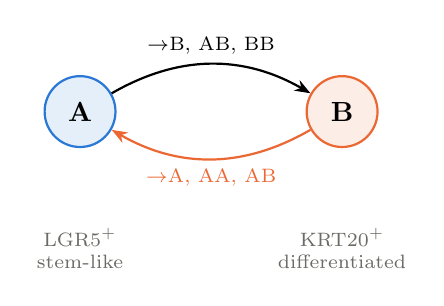
\begin{tikzpicture}[>={Stealth[length=2mm]},node distance=2.4cm,
  cell/.style={circle,draw,thick,minimum size=0.9cm,font=\bfseries}]
\node[cell,draw=cblue,fill=cblue!12] (A) {A};
\node[cell,draw=corange,fill=corange!12,right=of A] (B) {B};
\draw[->,thick] (A) to[bend left=30] node[above,font=\scriptsize]{$\to$B, AB, BB} (B);
\draw[->,thick,corange] (B) to[bend left=30] node[below,font=\scriptsize]{$\to$A, AA, AB} (A);
\node[below=0.9cm of A,font=\scriptsize,text=inkgray,align=center] {LGR5$^+$\\stem-like};
\node[below=0.9cm of B,font=\scriptsize,text=inkgray,align=center] {KRT20$^+$\\differentiated};
\end{tikzpicture}

\medskip
{\small Biological question: does \textbf{B} ever give rise to \textbf{A}?}
\end{column}
\end{columns}
\end{frame}

\begin{frame}{Probability generating functions}
One generation of a single cell, $s$ marks A daughters, $t$ marks B daughters:
\[
f_A(s,t) = p^A_{\rm d} + p^A_{\rm p}\,s + p^A_{\to B}\,t + p^A_{AA}\,s^2 + p^A_{AB}\,st + p^A_{BB}\,t^2,
\]
\[
f_B(s,t) = p^B_{\rm d} + p^B_{\rm p}\,t + p^B_{\to A}\,s + p^B_{AA}\,s^2 + p^B_{AB}\,st + p^B_{BB}\,t^2.
\]
Cells act independently, so after $g$ generations the clone's pgf is the \textbf{$g$-fold iterate}
\[
F_g = f \circ F_{g-1},\qquad F_0(s,t) = (s,t),
\]
\[
F^A_g(s,t) = \mathbb E\big[s^{A_g}t^{B_g}\mid \text{one A founder}\big] = \sum_{a,b} p(a,b\mid\theta,g)\, s^a t^b .
\]
\take{The whole distribution of $(A_g, B_g)$ is encoded in a function we can evaluate cheaply at any point $(s,t)$: $g$ compositions of two quadratic polynomials.}
\end{frame}

\begin{frame}{From the pgf to the exact likelihood}
\begin{columns}[T]
\begin{column}{0.56\textwidth}
\begin{enumerate}
\item Evaluate $F^A_g$ on a grid of \textbf{damped roots of unity}\\ $s_j = r_x e^{2\pi i j/L_x}$, $t_k = r_y e^{2\pi i k/L_y}$.
\item A \textbf{2-D inverse FFT} returns $p(a,b\mid\theta,g)$ for all $a<L_x$, $b<L_y$ at once (Cauchy coefficient formula).
\item Condition on detection: $P(\text{det}) = 1 - F^A_g(0,0)$.
\end{enumerate}
\[
\ell(\theta) = \sum_{g}\sum_{\text{clones } i}\Big[\log p(a_i,b_i\mid\theta,g) - \log P(\text{det}\mid\theta,g)\Big]
\]
\end{column}
\begin{column}{0.40\textwidth}\small
\begin{itemize}
\item grid sized from the data (largest $\approx 270\times420$ at gen.\ 10)
\item damping bounds round-off amplification by $10^4$; relative error $\le 10^{-6}$ vs a $2\times$ grid
\item clones grouped into a histogram: cost almost \textbf{independent of $n$}
\item exact gradients by differentiating through the recursion (reverse mode): \textbf{3--9\,ms} per log-likelihood + gradient
\end{itemize}
\end{column}
\end{columns}
\take{Exact, fast and differentiable $\Rightarrow$ we can use gradient-based optimisation and Hamiltonian Monte Carlo directly on the raw counts.}
\end{frame}

% ================================================================== 2 inference
\section{Inference: MLE and NUTS}

\begin{frame}{Two estimators on the same likelihood}
\begin{columns}[T]
\begin{column}{0.48\textwidth}
\textbf{Maximum likelihood}
\begin{itemize}\small
\item multistart L-BFGS-B in stick-breaking coordinates (29 starts)
\item standard errors from the observed Fisher information
\item \textbf{profile likelihood} for one parameter: fix it, maximise over the other 9
\end{itemize}
\smallskip
{\scriptsize\begin{tabular}{@{}lrr@{}}\toprule
global optimiser (30 problems) & hits & time \\\midrule
\textbf{multistart L-BFGS-B} & 27 & 0.8\,s \\
Adam + L-BFGS-B polish & 29 & 5.4\,s \\
PSO + L-BFGS-B & 25 & 4.4\,s \\
PSO / Adam alone & 7 / 12 & 4--5\,s \\\bottomrule
\end{tabular}}
\end{column}
\begin{column}{0.48\textwidth}
\textbf{Bayesian posterior: NUTS}
\begin{itemize}\small
\item 4 chains $\times$ (500 warm-up + 500 draws), dense mass matrix, logit-stick coordinates
\item starts: 16 prior draws $\to$ L-BFGS on the log posterior; chain $c$ starts near the $c$-th best optimum (Laplace draw)
\item checks: split $\hat R$, ESS, divergences, per-chain means
\item other priors by Pareto-smoothed importance reweighting
\end{itemize}
\smallskip
{\small\textbf{It works:} 99/108 runs mixed (median min ESS 276); Monte Carlo error $\approx 0.05$ posterior sd. The rest: posteriors with two branches.}
\end{column}
\end{columns}
\take{The sampler is not the bottleneck: what limits us is what the data contain.}
\end{frame}

% ================================================================== 3 setting
\section{Experimental setting}

\begin{frame}{Ground truths: curated (T) and drawn from the prior (P)}
\centering{\footnotesize\setlength{\tabcolsep}{5pt}
\begin{tabular}{@{}lllrl@{}}\toprule
truth & A row$^\dagger$ & B row$^\dagger$ (\BA{} in bold) & cells$^\ast$ & what it tests \\\midrule
T1 reference & .03 .03 .05 .55 .05 .29 & .10 .10 \textbf{.80} 0 0 0 & 96 & B switches back, never divides \\
T2 & as T1 & .25 .25 \textbf{.50} 0 0 0 & 56 & weaker switch back \\
T4 slow A & .06 .06 .06 .40 .10 .32 & as T1 & 45 & less A self-renewal \\
T3 B divides & as T1 & .10 .08 \textbf{.60} .02 .05 .15 & 118 & interior truth \\
T5 large clones & .05 .10 .10 .50 .15 .10 & .08 .05 \textbf{.10} .05 .05 .67 & 196 & B self-renews \\\midrule
P1 & .10 .06 .30 .12 .34 .08 & .19 .15 \textbf{.11} .26 .27 .02 & 31 & \multirow{4}{*}{draws from the prior} \\
P2 & .29 .13 .01 .31 .04 .23 & .03 .13 \textbf{.12} .35 .00 .36 & 39 & \\
P3 & .04 .14 .10 .12 .21 .40 & .08 .04 \textbf{.27} .20 .33 .08 & 120 & \\
P4 & .22 .05 .06 .37 .28 .03 & .06 .13 \textbf{.11} .18 .51 .02 & 61 & \\\bottomrule
\end{tabular}}

\raggedright{\scriptsize $^\dagger$ order: death, persist, switch, AA, AB, BB.\quad $^\ast$ expected living cells per clone at generation 10.}
\end{frame}

\begin{frame}{The XG2 experiment: data size}
\begin{columns}[T]
\begin{column}{0.55\textwidth}
\begin{itemize}
\item endpoints: generations \textbf{4, 6, 8, 10} jointly
\item $n$ = \textbf{128, 256, 512, 1024} clones per endpoint\\ (+ 2048, 4096 for T1--T4)
\item 3 datasets per truth, \textbf{nested} across $n$: each (truth, dataset) is one convergence curve
\item all 10 probabilities free, flat prior
\item for every run: NUTS posterior + MLE (+ profiles, other priors)
\end{itemize}
\end{column}
\begin{column}{0.40\textwidth}
\begin{block}{Size}
\small 9 truths $\times$ 3 datasets $\times$ 4 sizes = \textbf{108 posteriors}\\
+ 24 large-$n$ runs\\
+ 108 under each alternative prior\\[3pt]
0.1--4\,h per run
\end{block}
\begin{block}{Reference point}
\small real CRC0322 data: days 6 and 10,\\ 165 and 101 organoids
\end{block}
\end{column}
\end{columns}
\end{frame}

% ================================================================== 4 convergence
\section{Convergence and data size}

\begin{frame}{A's row converges fast, B's row does not}
\centering
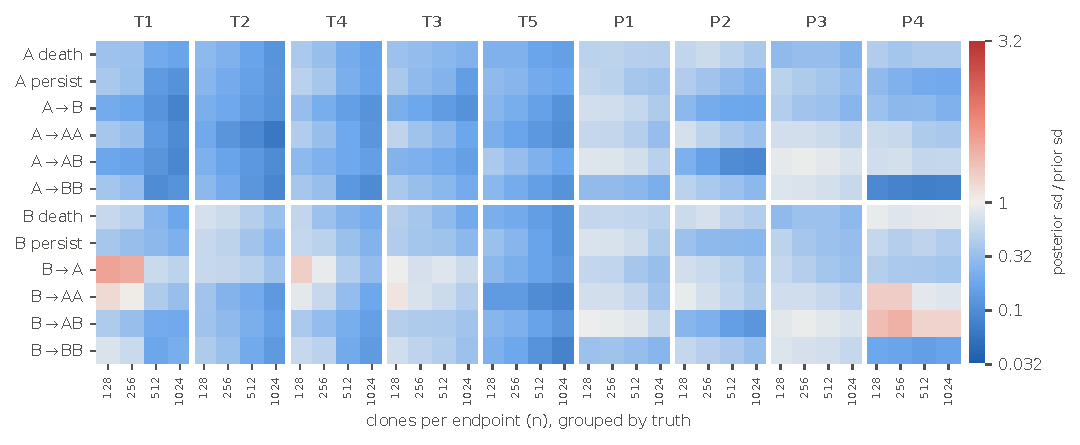
\includegraphics[width=0.97\textwidth]{contraction.pdf}
\vspace{-2pt}
{\small Posterior sd / prior sd (blue = narrowed, white = prior-like, red = wider than the prior).
A's row: $3$--$10\times$ narrower at $n$ = 128, $10$--$30\times$ at 1024. T5 (large clones): everything $\ge 2.4\times$ at 128.}
\end{frame}

\begin{frame}{B$\to$A against $n$}
\begin{columns}[c]
\begin{column}{0.55\textwidth}
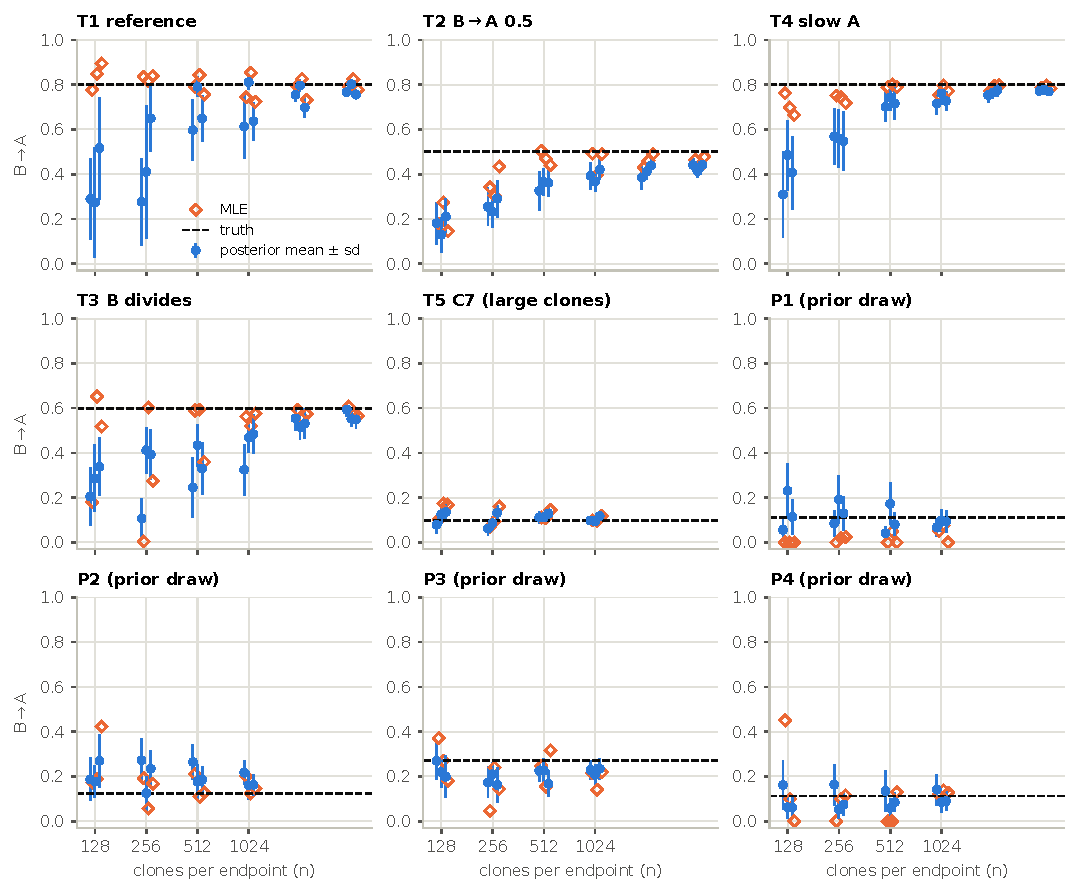
\includegraphics[width=\textwidth]{btoa_vs_n.pdf}
\end{column}
\begin{column}{0.43\textwidth}
{\scriptsize\setlength{\tabcolsep}{2.5pt}
\begin{tabular}{@{}lrrrrr@{}}\toprule
 & truth & 128 & 256 & 512 & 1024 \\\midrule
T1 post. & .80 & .36 & .45 & .68 & .69 \\
\phantom{T1} MLE & & .84 & .83 & .80 & .77 \\
T2 post. & .50 & .17 & .26 & .35 & .39 \\
\phantom{T2} MLE & & .20 & .36 & .47 & .46 \\
T3 post. & .60 & .28 & .30 & .34 & .43 \\
\phantom{T3} MLE & & .45 & .29 & .51 & .55 \\
T5 post. & .10 & .11 & .09 & .12 & .10 \\\bottomrule
\end{tabular}}
\begin{itemize}\small
\item large \BA: posterior mean \alert{1--2 sd low}, same sign in every dataset
\item small \BA{} (T5, P1--P4): recovered at every $n$
\item MLE tracks large \BA{} from $n$ = 256
\end{itemize}
\end{column}
\end{columns}
\end{frame}

\begin{frame}{How much data until B's row converges?}
\begin{columns}[c]
\begin{column}{0.52\textwidth}
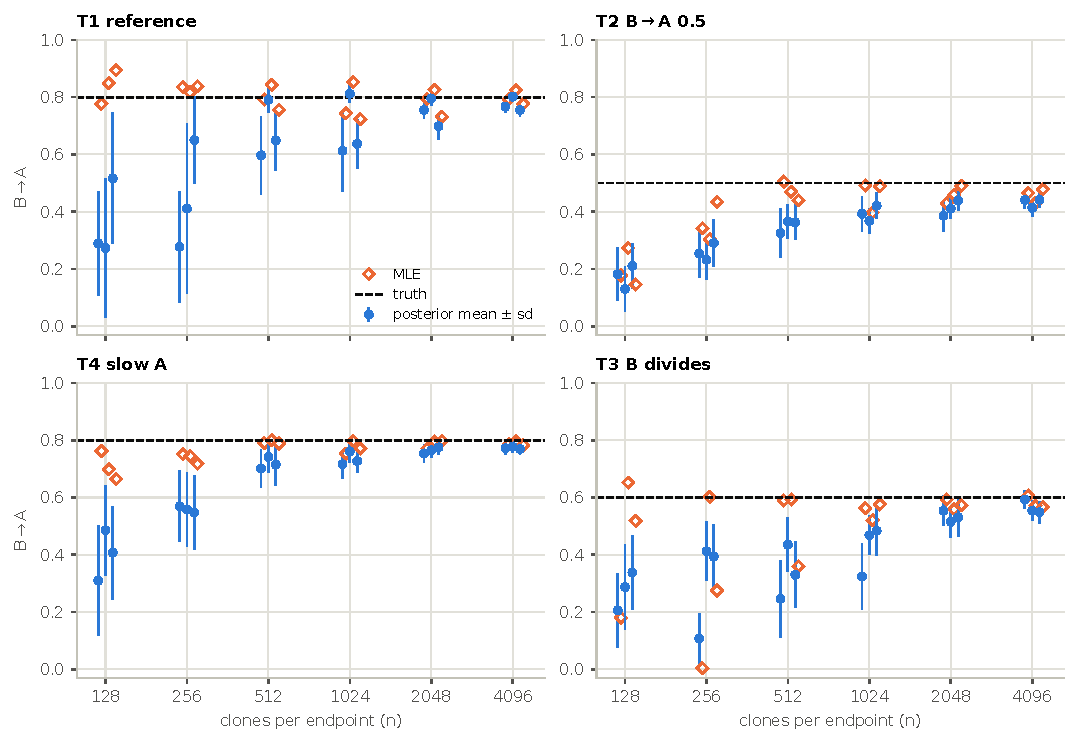
\includegraphics[width=\textwidth]{btoa_large_n.pdf}
\end{column}
\begin{column}{0.45\textwidth}\small
\begin{itemize}
\item \BA{} within 0.05 of the truth at \textbf{2048--4096} clones per endpoint (T2 not even at 4096); the MLE one doubling earlier
\item but where B never divides, the posterior stays \textbf{1--2 sd low at every $n$}
\item at 1024 the answer still moves by 0.2--1.2 sd when the prior changes
\item A's row, growth rate and composition: $n^{-1/2}$ regime from 256--512
\end{itemize}
\take{Rule of thumb: A's row needs $\sim$300, B's row needs thousands of clones per endpoint with the current design.}
\end{column}
\end{columns}
\end{frame}

\begin{frame}{MLE or posterior mean?}
\begin{columns}[c]
\begin{column}{0.48\textwidth}
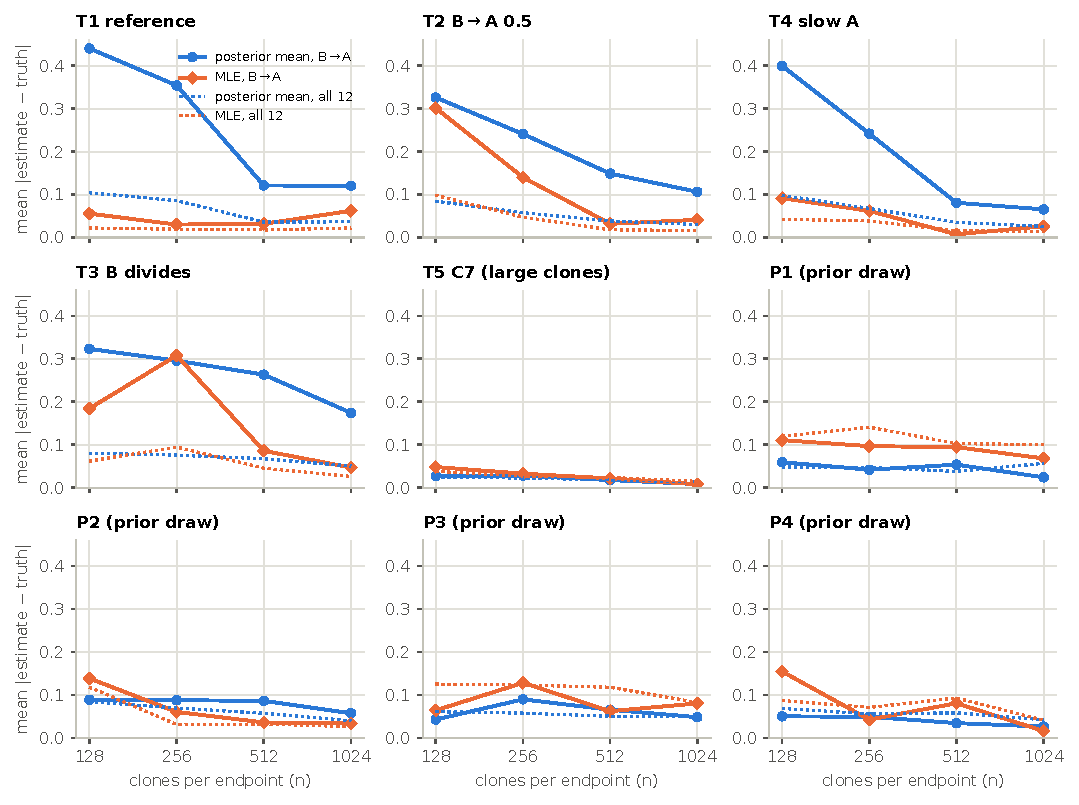
\includegraphics[width=\textwidth]{mle_vs_posterior.pdf}
\end{column}
\begin{column}{0.50\textwidth}\small
\begin{itemize}
\item \textbf{Large \BA{}} (T1--T4): MLE error 0.01--0.06, posterior mean 0.07--0.44
\item \textbf{Prior draws, small $n$}: posterior mean better (MLE jumps between near-equal optima, often exactly 0)
\item posterior error for B's row is mostly \textbf{bias}: RMSE / posterior sd = 1.5--2.0 at 128, 1.3--1.6 at 1024 $\Rightarrow$ \alert{overconfident}
\item truth inside the 95\% likelihood region in 107/108 runs
\end{itemize}
\take{Neither dominates. Report likelihood-based intervals next to posterior ones.}
\end{column}
\end{columns}
\end{frame}

% ================================================================== 5 hardest
\section{Which parameters are hard}

\begin{frame}{Ranking the 12 probabilities (all truths, flat prior)}
\begin{columns}[c]
\begin{column}{0.58\textwidth}
{\scriptsize\setlength{\tabcolsep}{3.5pt}
\begin{tabular}{@{}rlrrrrr@{}}\toprule
 & & \multicolumn{3}{c}{RMSE posterior mean} & 90\% & RMSE \\
 & parameter & $n$=128 & 512 & 1024 & cover. & MLE 1024 \\\midrule
12 & \alert{\textbf{B$\to$A}} & \textbf{.260} & \textbf{.127} & \textbf{.095} & \textbf{.60} & .055 \\
11 & B$\to$AA & .155 & .088 & .058 & .81 & .072 \\
10 & B$\to$AB & .103 & .081 & .078 & .88 & .099 \\
9 & B$\to$BB & .088 & .057 & .053 & .93 & .057 \\
8 & A$\to$BB & .067 & .048 & .046 & .82 & .050 \\
7 & A death & .084 & .055 & .044 & .81 & .026 \\
6 & B death & .088 & .067 & .060 & .93 & .036 \\
5 & A$\to$AB & .050 & .044 & .056 & .96 & .083 \\
4 & B persist & .063 & .039 & .041 & .94 & .055 \\
3 & A$\to$AA & .057 & .037 & .033 & .91 & .056 \\
2 & A persist & .059 & .037 & .027 & .94 & .044 \\
1 & A$\to$B & .042 & .040 & .031 & .94 & .054 \\\bottomrule
\end{tabular}}

{\tiny Every probability has prior sd 0.141 (Beta(1,5) marginal), so errors are comparable.}
\end{column}
\begin{column}{0.40\textwidth}\small
\begin{itemize}
\item \textbf{\BA{} is the hardest} on 6 of 7 measures; 90\% intervals cover only 35\% for T1--T4
\item then B's three divisions
\item A's row is easy: within $\approx 0.03$ at 1024
\item exception: the \textbf{MLE} estimates \BA{} about as well as most parameters
\end{itemize}
\take{\BA{} is both the hardest parameter and the biological question.}
\end{column}
\end{columns}
\end{frame}

\begin{frame}{Why are B's parameters hard?}
\begin{columns}[c]
\begin{column}{0.50\textwidth}
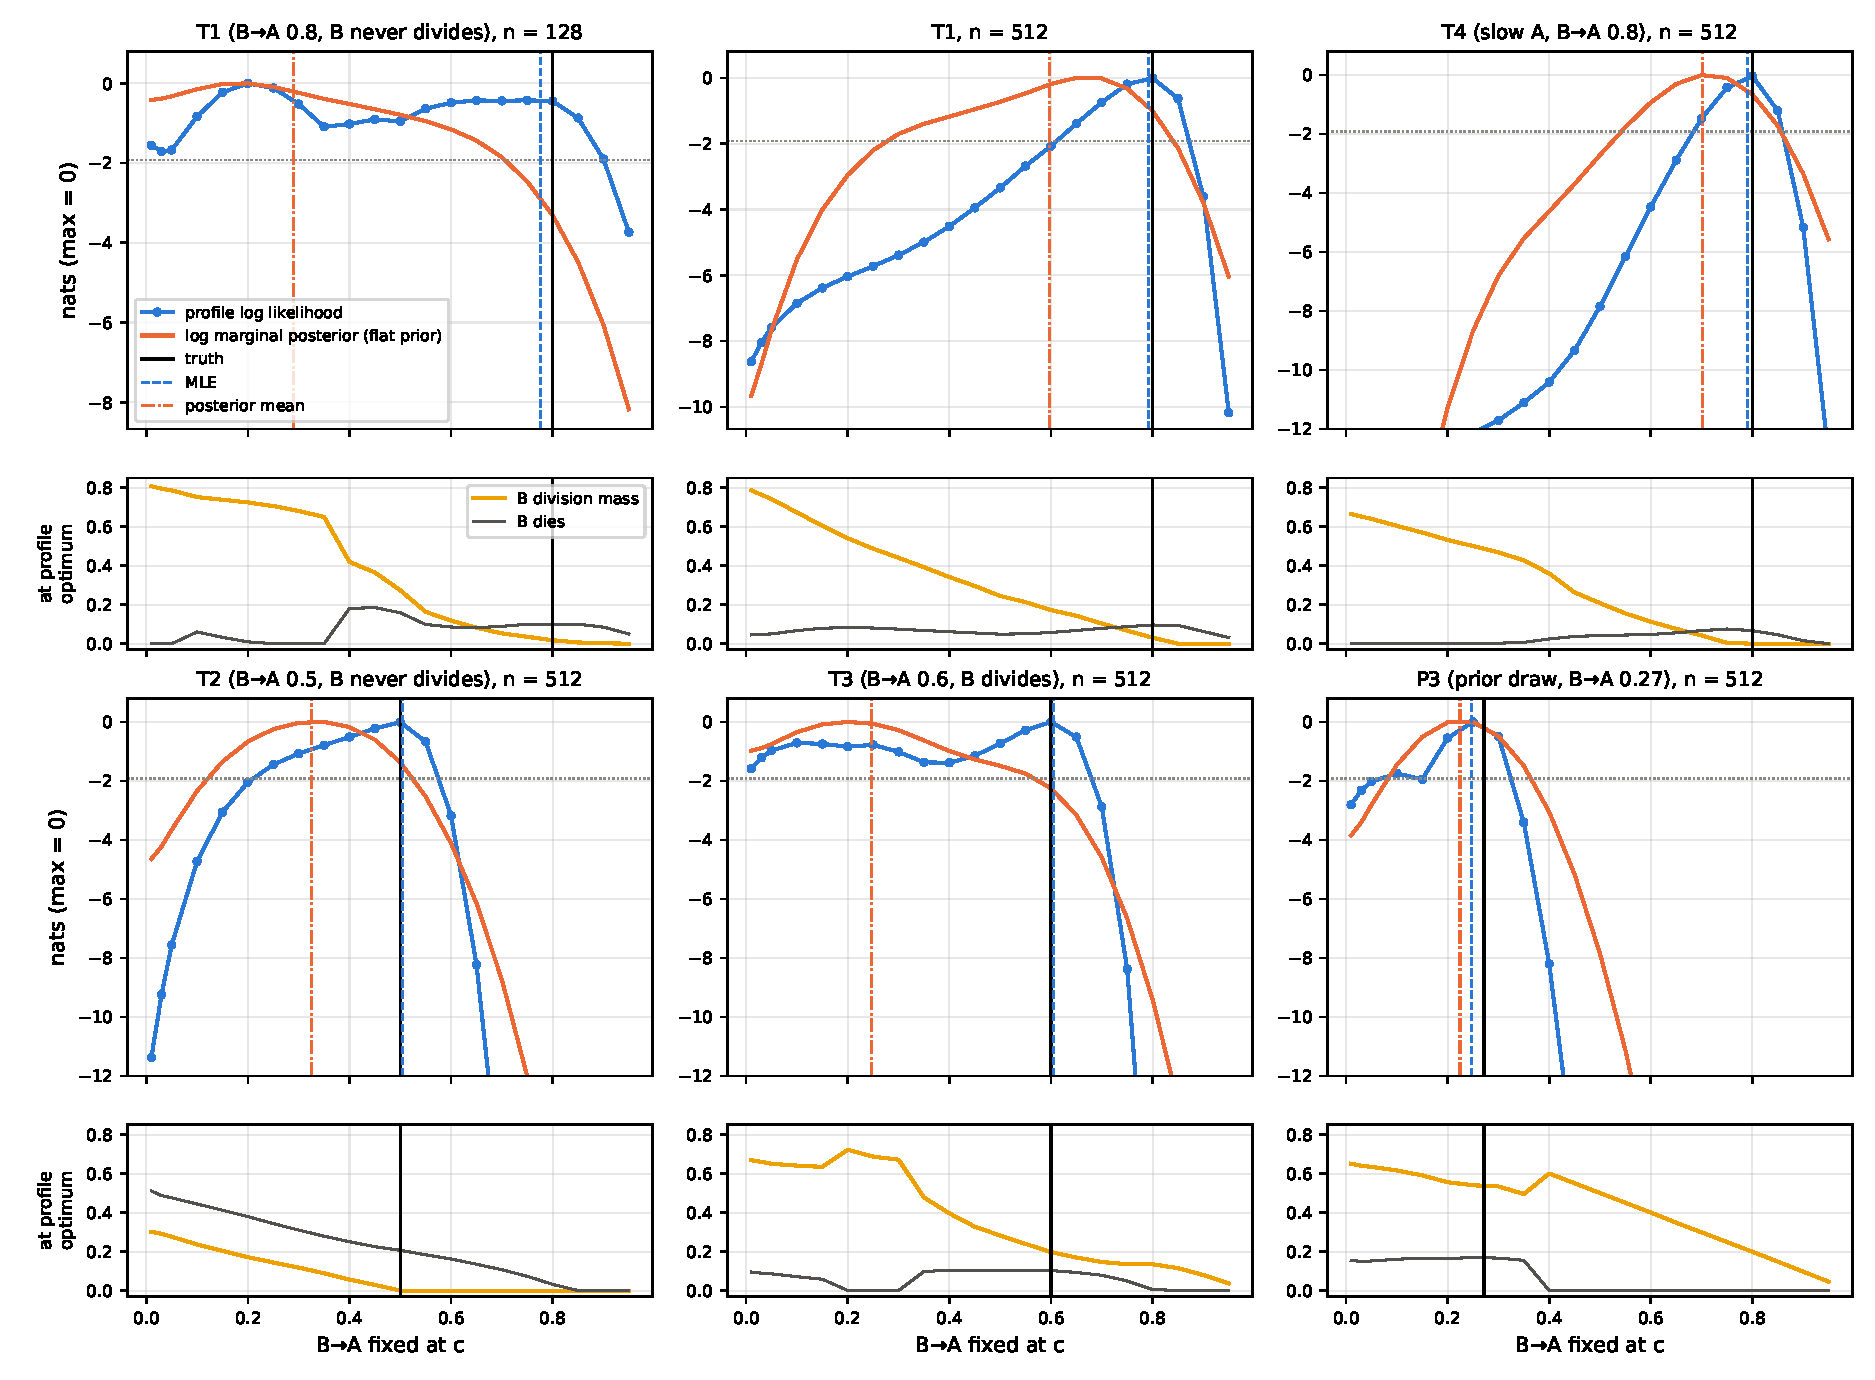
\includegraphics[width=\textwidth]{profile_panels.pdf}
\end{column}
\begin{column}{0.48\textwidth}\small
\begin{enumerate}
\item \textbf{A founds every clone}: B's behaviour is seen only inside mixed populations, never in isolation.
\item \textbf{Compensation}: ``B switches back to A'' and ``B is lost'' (dies, or divides into B's) give almost the same counts $\Rightarrow$ flat, often two-branched likelihood (blue).
\item \textbf{Boundaries}: ``B never divides'' is a face of the simplex; posteriors are truncated there.
\item \textbf{Small clones} carry little information (T5, $\sim$200 cells, is easy).
\end{enumerate}
{\scriptsize Blue: profile log-likelihood of \BA; orange: log marginal posterior. T1 at $n$=128: the profile drops only 1.9 nats from \BA{} = 0.9 to 0.2.}
\end{column}
\end{columns}
\end{frame}

% ================================================================== 6 bias
\section{The bias of B$\to$A}

\begin{frame}{Where the bias comes from: prior volume on a flat ridge}
\centering
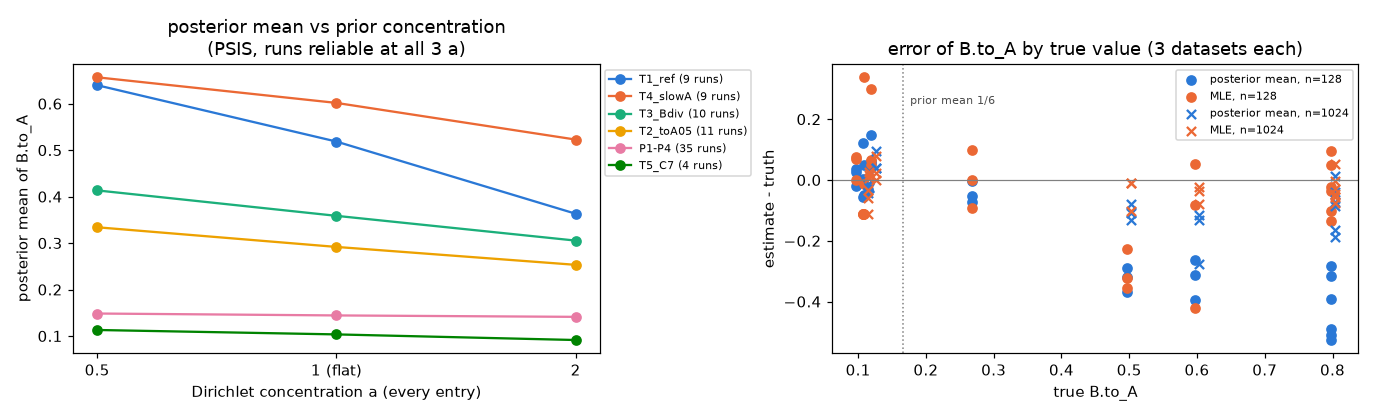
\includegraphics[width=0.84\textwidth]{prior_alpha_and_bias.png}

\vspace{-2pt}
\begin{columns}[T]
\begin{column}{0.57\textwidth}\footnotesize
\begin{itemize}
\item \textbf{Left}: same data, only the prior changes. Larger $a$ puts more volume at small \BA{} $\Rightarrow$ lower posterior mean (39/39 runs of T1--T4).
\item \textbf{Right}: for large true \BA{} the posterior mean is \textbf{always too low}, by up to 0.5; the MLE (orange) is mostly closer, and near 0 by $n$=1024.
\item Flat Dirichlet: \BA{} $\sim$ Beta(1,\,5), mean 1/6. On the flat ridge (``B switches back'' vs ``B is lost'') this volume decides.
\end{itemize}
\end{column}
\begin{column}{0.40\textwidth}
\begin{block}{Coverage of \BA{} (13 profiled runs)}
\footnotesize 95\% \textbf{profile-likelihood} interval: \textbf{13/13}\\
95\% posterior interval: \alert{5/13}, every miss on the low side
\end{block}
{\scriptsize Not only boundary truths: T3 (interior) is as biased as T1.}
\end{column}
\end{columns}
\end{frame}

\begin{frame}{The bias does not go away with more data or another prior}
\begin{columns}[T]
\begin{column}{0.44\textwidth}\small
\textbf{Boundary:} at a face of the simplex the posterior is a truncated normal: its bias stays a fixed number of sds. T1, T2, T4: mean $z$ = $-1.2$ to $-2.4$ at every $n$ up to 4096.

\medskip
\textbf{Other ``uninformative'' priors} (all 108 cells):
\begin{itemize}
\item Dirichlet($\tfrac12$): best symmetric prior, bias remains
\item exact Jeffreys prior: proper, but concentrates on \BA{} $\approx 0$ and B self-renewal
\item flat prior on \BA{} only: fixes large \BA, doubles the error of small \BA{} at $n$=128
\end{itemize}
\end{column}
\begin{column}{0.54\textwidth}
{\scriptsize\setlength{\tabcolsep}{3pt}
\begin{tabular}{@{}llrrrrr@{}}\toprule
 & $n$ & unif.\ Dir & flat-\BA & Dir($\tfrac12$) & Jeffreys & MLE \\\midrule
RMSE \BA & 128 & .260 & \textbf{.137} & .188 & .210 & .172 \\
 & 1024 & .095 & \textbf{.043} & .071 & .075 & .055 \\
bias \BA & 128 & $-$.158 & $-$.014 & $-$.096 & $-$.131 & $-$.039 \\
 & 1024 & $-$.053 & $-$.003 & $-$.035 & $-$.044 & $-$.026 \\
90\% cov. & 1024 & .63 & .89 & .78 & .67 & .81 \\\bottomrule
\end{tabular}}
\take{At $n \le 1024$ no ``uninformative'' prior is neutral about \BA: the estimate moves by more than its sd when the prior changes. Report prior-free quantities (MLE, profile, LR test) or a range over priors.}
\end{column}
\end{columns}
\end{frame}

\begin{frame}{The fix: first ask ``does B divide?''}
\begin{columns}[c]
\begin{column}{0.45\textwidth}
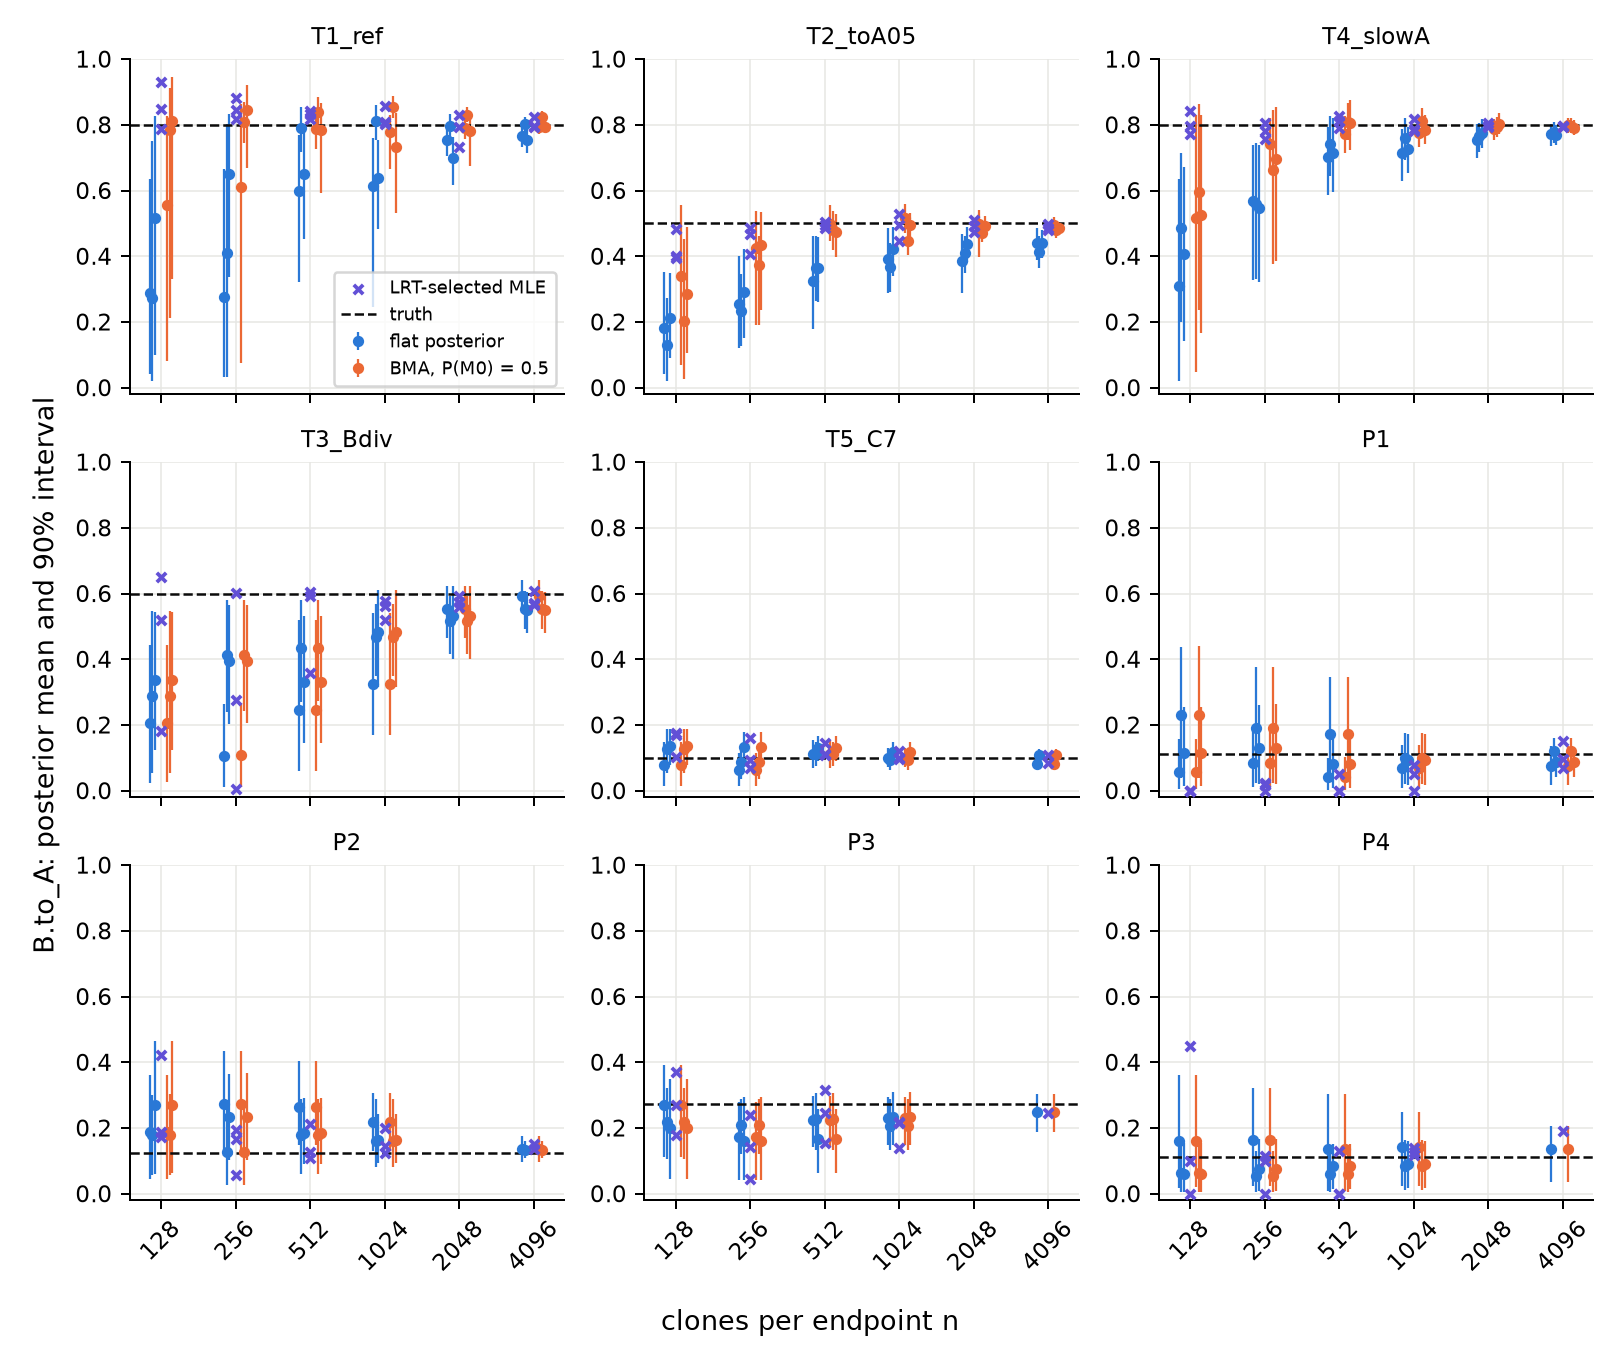
\includegraphics[width=\textwidth]{btoa_bma_vs_flat.png}
\end{column}
\begin{column}{0.53\textwidth}\small
\textbf{Spike-and-slab prior}: probability $\tfrac12$ on ``B never divides'' (B$\to$AA = AB = BB = 0), $\tfrac12$ on the full model; evidences by bridge sampling.

\smallskip
{\scriptsize\setlength{\tabcolsep}{2.5pt}
\begin{tabular}{@{}lrrr@{}}\toprule
\BA, T1/T2/T4 (54 runs) & RMSE & cover.\ 95\% & mean $z$ \\\midrule
flat posterior & 0.218 & 0.41 & $-1.88$ \\
model average, P(M$_0$) = 0.5 & \textbf{0.099} & \textbf{0.89} & $-0.39$ \\
MLE of LRT-selected model & 0.040 & --- & --- \\\bottomrule
\end{tabular}}
\begin{itemize}
\item P(B never divides $\mid$ data) = 0.92--0.97 at $n$=512 when true; $\le 0.004$ when false
\item LR test picks the right model in \textbf{37/37} runs already at $n$=128
\item \textbf{no cost} where B divides; does not help T3 (interior)
\end{itemize}
\end{column}
\end{columns}
\end{frame}

% ================================================================== 7 weak directions
\section{Weak directions}

\begin{frame}{What do the counts not tell apart? Fisher information}
\begin{columns}[c]
\begin{column}{0.60\textwidth}
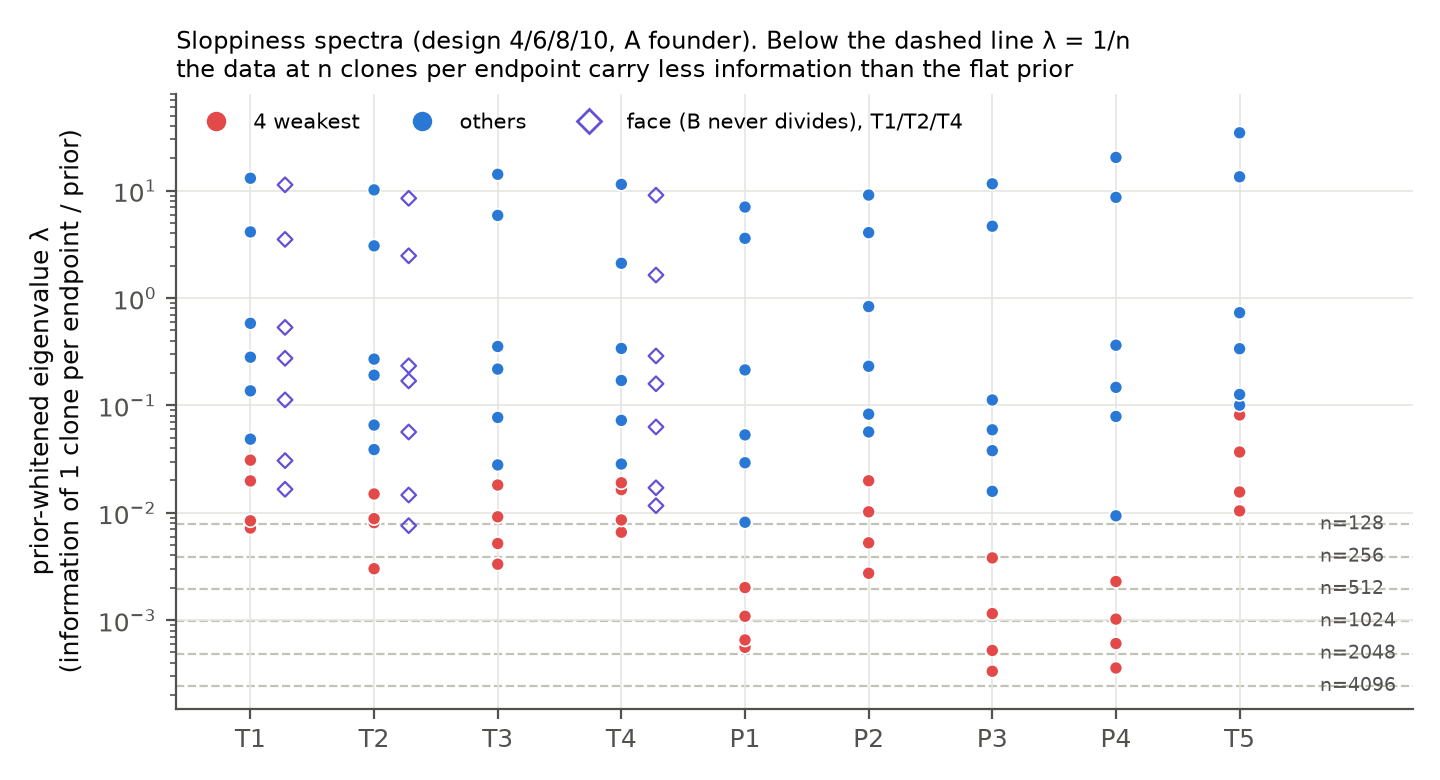
\includegraphics[width=\textwidth]{spectra.png}
\end{column}
\begin{column}{0.38\textwidth}\small
Eigen-decompose the exact Fisher information of one clone, scaled by the prior.\\
$1/\lambda$ = \textbf{clones per endpoint} at which the data match the prior along that direction.

\medskip
\textbf{Three tiers, in every truth}
\begin{itemize}
\item 2 directions need $<1$ clone: growth, offspring composition
\item 2--4 need 1--35 clones
\item \alert{4--5 weak}: 30--330 (T1--T4), 260--3000 (prior draws)
\end{itemize}
\end{column}
\end{columns}
\end{frame}

\begin{frame}{The weak directions are ``parent swaps''}
\begin{columns}[T]
\begin{column}{0.56\textwidth}
Move an outcome from A parents to B parents while the \textbf{average cell} (weighted by the stable A/B composition) does the same thing.

\smallskip
{\scriptsize\setlength{\tabcolsep}{3pt}
\begin{tabular}{@{}lrr@{}}\toprule
 & \multicolumn{2}{c}{clones/endpoint to halve var.} \\
swap: the counts cannot tell & T1--T4 & P1--P4 \\\midrule
whether A or B makes AB divisions & 67--155 & 109--2287 \\
whether A or B cells die & 34--79 & 270--2141 \\
switch vs persist (the \BA{} ridge) & 62--107 & 63--1023 \\
whether A or B makes AA vs BB & 33--85 & 117--542 \\
whether A or B cells divide & 30--66 & 22--120 \\\bottomrule
\end{tabular}}

\smallskip
{\small 35 of the 36 weakest directions lie in this 5-dim ``swap'' block.}
\end{column}
\begin{column}{0.42\textwidth}\small
\textbf{Why (Kesten--Stigum).} With mean offspring matrix $M$, growth rate $\rho$, stable composition $u$:
\[ u^\top \Delta M = (-u_Au_B + u_Bu_A)\,d^\top O = 0 \]
$\Rightarrow$ a swap leaves $\rho$ and $u$ \textbf{exactly} unchanged.\\
Grown clones sit at $u$ and grow at $\rho$, so they barely see swaps.

\medskip
\take{The counts record what the population does, not which type of cell did it.}
\end{column}
\end{columns}
\end{frame}

\begin{frame}{Example: which parent made the mixed division? (P3, $n$ = 1024)}
\centering
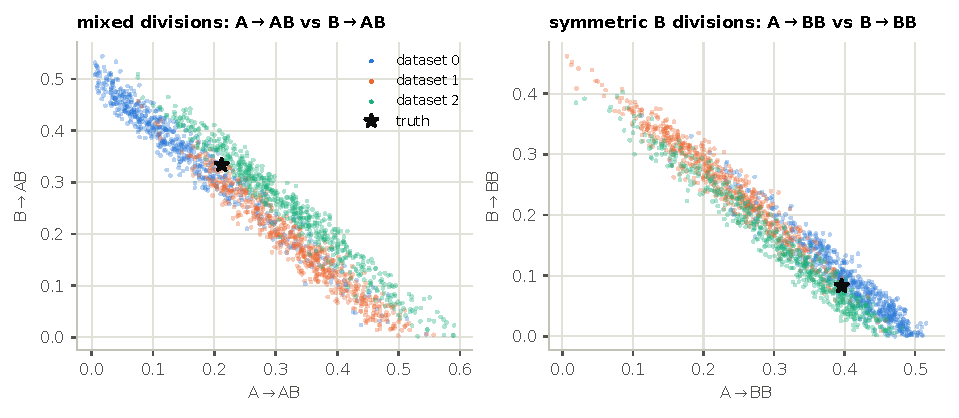
\includegraphics[width=0.88\textwidth]{p3_ridge.pdf}

\small
Three datasets, all converged, give different A$\to$AB (0.16 vs 0.34); corr.\ with B$\to$AB $= -0.98$.\\
Yet the \textbf{identifiable combinations agree}: growth $1.603 \pm .004$ vs $1.606 \pm .004$ (truth 1.609), stable A fraction 0.493 vs 0.495 (0.493).
\end{frame}

\begin{frame}{Where the information on weak directions comes from}
\centering
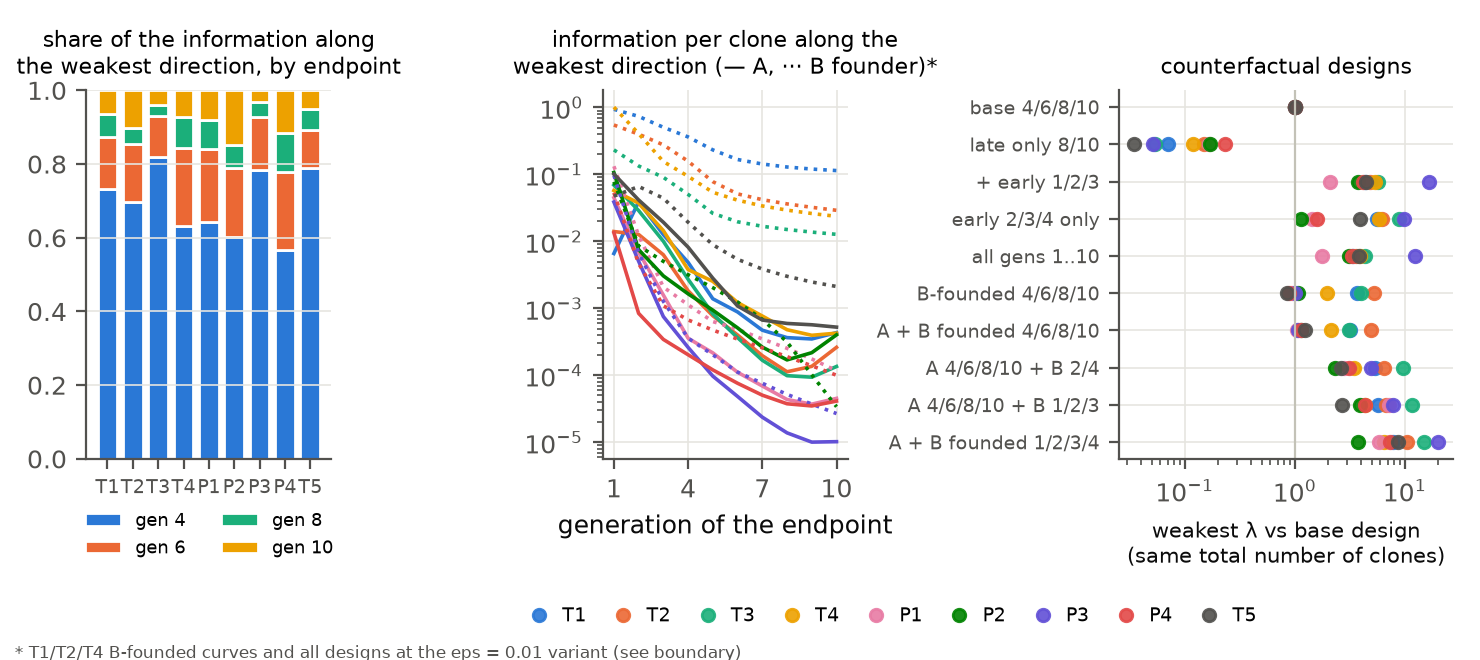
\includegraphics[width=0.78\textwidth]{generations_designs.png}

\begin{columns}[T]
\begin{column}{0.48\textwidth}\small
\begin{itemize}
\item generation 4 gives \textbf{57--91\%} of it; generation 10 only 1--15\%
\item early, a clone is all A: the parent of every event is known
\end{itemize}
\end{column}
\begin{column}{0.48\textwidth}\small
\begin{itemize}
\item information per clone falls like $\rho^{-h}$: \textbf{each later generation costs a factor $\rho \approx$ 1.4--1.7 in clones}
\item B-founded clones observe B's fate directly
\end{itemize}
\end{column}
\end{columns}
\end{frame}

% ================================================================== 8 dediff
\section{Testing for dedifferentiation}

\begin{frame}{A yes/no question instead of an estimate}
\begin{columns}[T]
\begin{column}{0.52\textwidth}
\textbf{Does B ever give rise to A, by any route?}
\[ m_{BA} = \text{B}{\to}\text{A} + 2\,\text{B}{\to}\text{AA} + \text{B}{\to}\text{AB} \]
= A cells produced per B cell per generation.

\medskip
\textbf{H0}: $m_{BA}=0$ (B dies, persists, or makes BB)\\
\textbf{H1}: dedifferentiation allowed
\[ \Lambda = 2\,[\ell(\hat\theta_{H1}) - \ell(\hat\theta_{H0})] \]
Under H0 some clones are nearly impossible (one A, no B at gen.\ 8: $p \approx 3\times10^{-7}$).
\end{column}
\begin{column}{0.45\textwidth}\small
\textbf{Calibration.} The tested probabilities sit on a boundary $\Rightarrow$ $\Lambda = 0$ in 25--77\% of null datasets; reference is a $\bar\chi^2$ mixture with \textbf{dataset-specific weights}.
\begin{itemize}
\item $\bar\chi^2$ from the fit: 1--6.5\% false positives at nominal 5\%
\item textbook $\chi^2_3$: too strict
\item a fixed threshold from a table: up to 16\% false positives
\end{itemize}
\take{Perfect typing: detects $m_{BA}\approx 0.003$ with 128 clones per endpoint --- about \textbf{26 events} in the whole experiment.}
\end{column}
\end{columns}
\end{frame}

\begin{frame}{Power, and the catch: cell-typing errors}
\begin{columns}[c]
\begin{column}{0.46\textwidth}
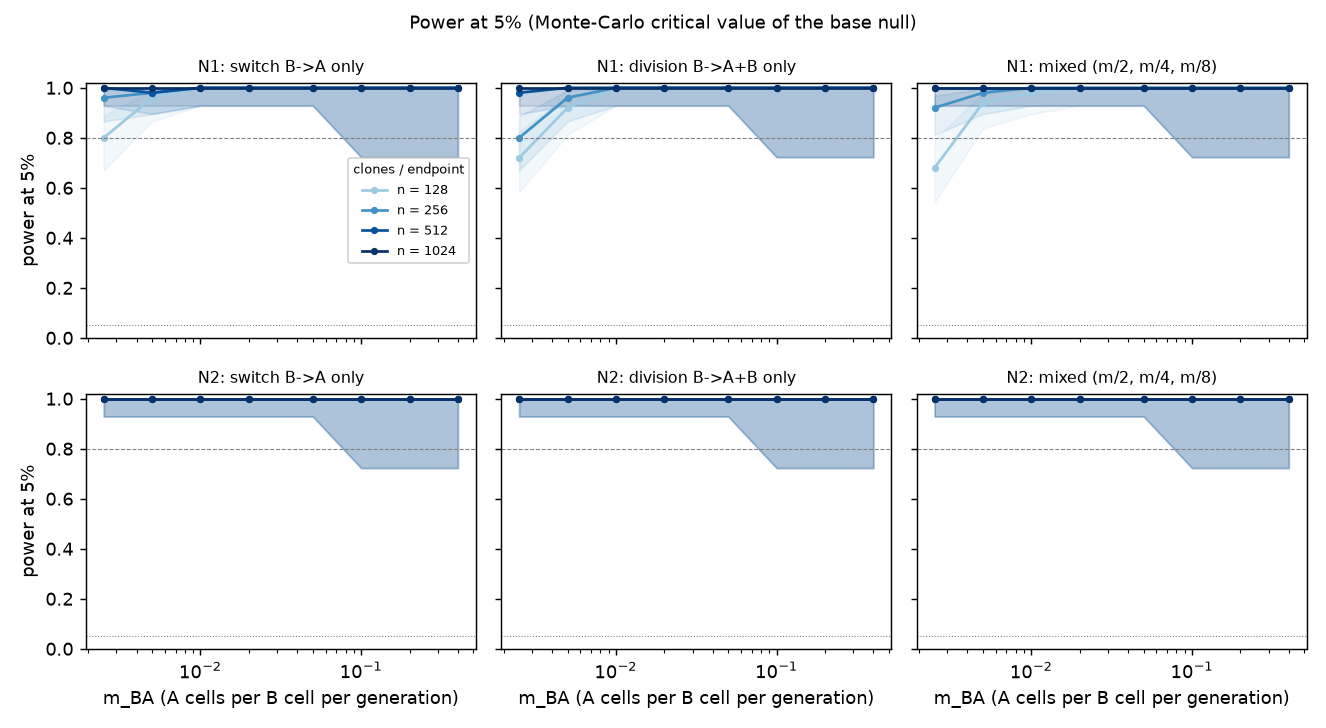
\includegraphics[width=\textwidth]{power_mc.png}
\end{column}
\begin{column}{0.52\textwidth}\small
A KRT20$^+$ cell scored LGR5$^+$ looks \textbf{exactly} like dedifferentiation. At 0.5\% mis-scoring, $\approx$15 misread cells vs 26 true events.

\smallskip
{\scriptsize\begin{tabular}{@{}ll@{}}\toprule
error rate used in the analysis & false positives \\\midrule
ignored & \alert{75--100\%} \\
10--20\% too low & \alert{up to 93\%} \\
exact & 1--13\% \\
50--100\% too high & $\le$ 4\%, little power lost \\\bottomrule
\end{tabular}}

\smallskip
\textbf{Robust test}: give a measured interval for the rate; reject only if rejected at every rate in it.

\smallskip
{\scriptsize Real CRC0322 data: $\Lambda = 45$, $p$ = 0.005, but $\hat m_{BA}$ = 1.35 is implausible: typing errors and organoid heterogeneity are not modelled $\Rightarrow$ \textbf{not evidence}.}
\end{column}
\end{columns}
\end{frame}

% ================================================================== 9 wet lab
\section{Ideas for the wet lab}

\begin{frame}{Optimal design: observe early, found some clones with B}
\begin{columns}[c]
\begin{column}{0.40\textwidth}
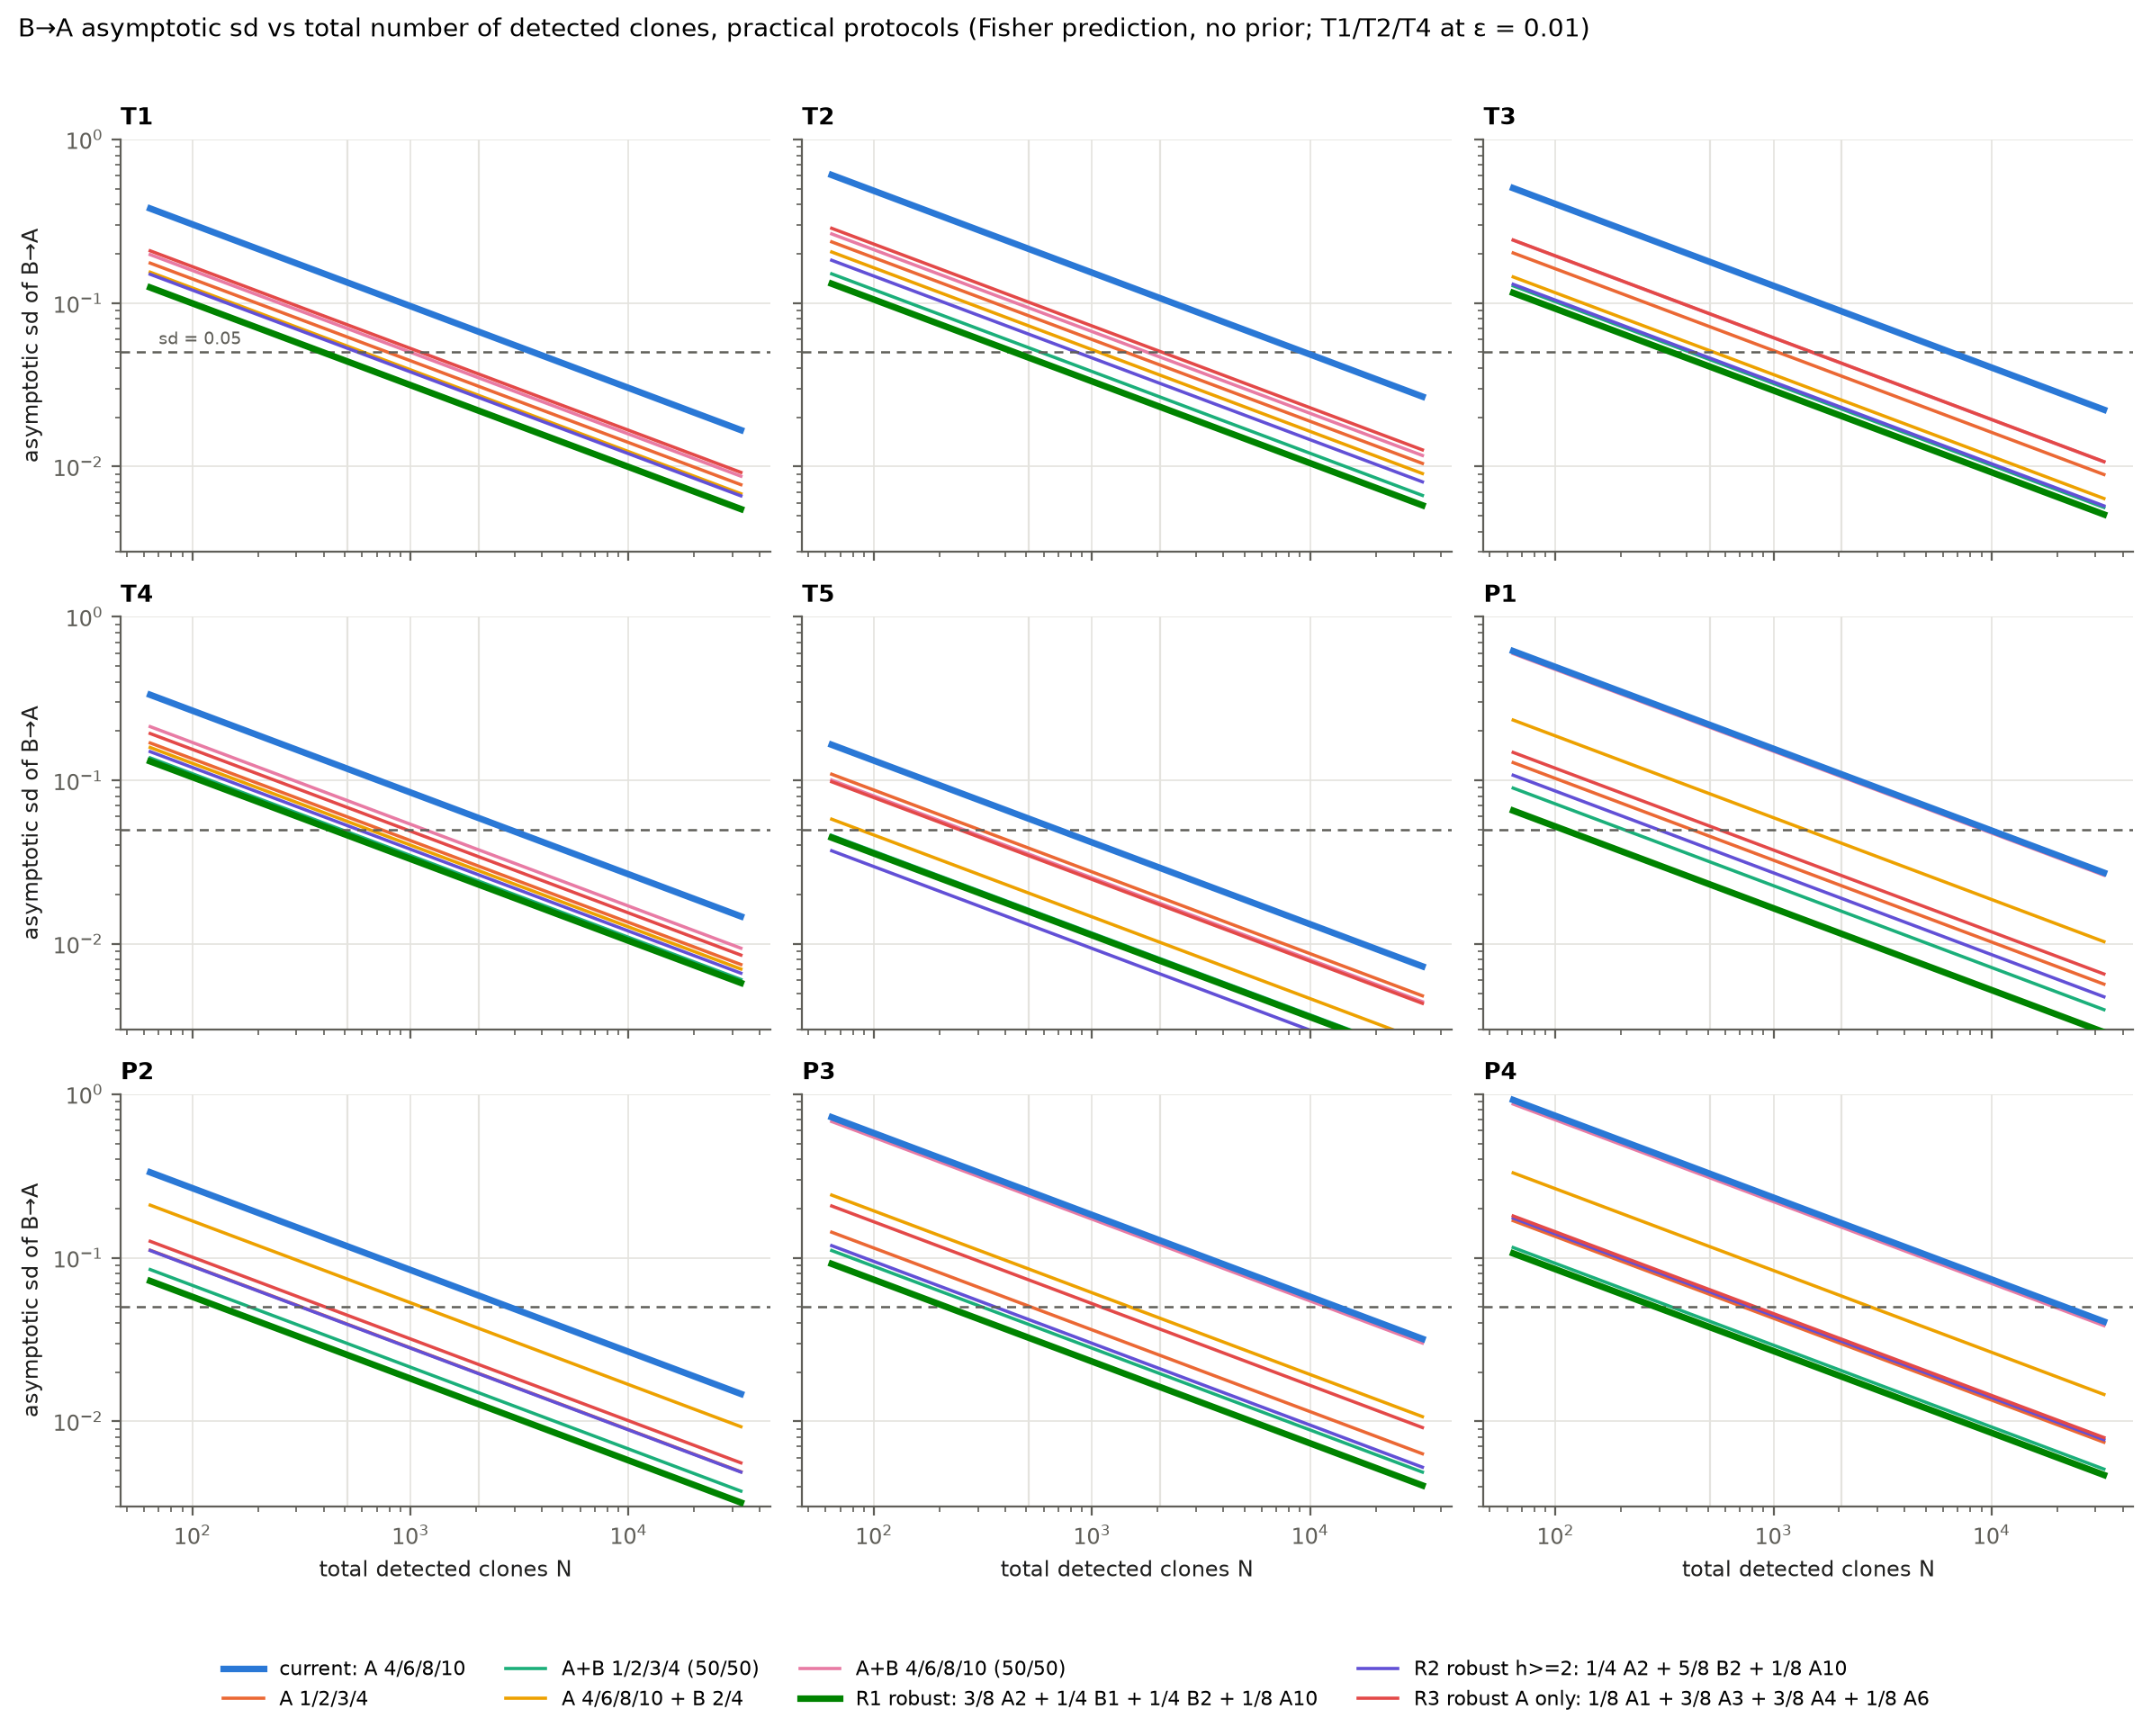
\includegraphics[width=\textwidth]{btoa_sd_vs_N.png}
\end{column}
\begin{column}{0.58\textwidth}
{\scriptsize\setlength{\tabcolsep}{3pt}
\begin{tabular}{@{}lrr@{}}\toprule
protocol: founder + generation & var.\ gain & clones for sd(\BA) $\le$ .05 \\\midrule
current: A at 4/6/8/10 & 1 & 700--21\,700 \\
A at 1/2/3/4 & 6.6 & 300--1\,430 \\
A+B at 1/2/3/4 & 16 & 54--580 \\
\textbf{R1}: $\tfrac38$A2 + $\tfrac14$B1 + $\tfrac14$B2 + $\tfrac18$A10 & \textbf{21} & \textbf{51--440} \\
R2 (no gen.\ 1): $\tfrac14$A2 + $\tfrac58$B2 + $\tfrac18$A10 & 15 & 35--850 \\
R3 (no B sort): A at 1/3/4/6 & 4.5 & 250--2\,100 \\\bottomrule
\end{tabular}}

\smallskip
\small
\begin{itemize}
\item optimum: 88--99\% of clones at generations 1--3, $\sim$5\% late (pins the growth rate)
\item checked by simulated MLEs: early designs match the prediction; the current design is $1.4\times$ \emph{worse} than predicted
\end{itemize}
\end{column}
\end{columns}
\end{frame}

\begin{frame}{Concrete suggestions for the lab}
\begin{columns}[T]
\begin{column}{0.49\textwidth}
\begin{block}{1. Organoids from single sorted KRT20$^+$ cells}
\small Observes B's fate directly. Any validated LGR5$^+$ cell is direct evidence of dedifferentiation.
\end{block}
\begin{block}{2. Early time points (1--2 divisions)}
\small Score clones at a \emph{known} number of divisions: match the time point to the cell cycle, or count divisions (live imaging).
\end{block}
\begin{block}{3. Keep one late endpoint}
\small $\sim$1/8 of clones at a late generation pins growth and composition.
\end{block}
\end{column}
\begin{column}{0.49\textwidth}
\begin{alertblock}{4. Measure the typing error on the same assay}
\small P(KRT20$^+$ scored LGR5$^+$): an \textbf{upper limit} to $\pm$25\% $\approx$ 3\,000 KRT20$^+$ cells of known identity (2\% error), e.g.\ sorted pure populations or double staining.
\end{alertblock}
\begin{block}{5. Also record}
\small plating efficiency (empty clones), how many cells were seeded, organoid-to-organoid heterogeneity (fate differences, slowing growth).
\end{block}
\end{column}
\end{columns}
\end{frame}

% ================================================================== 10 the end
\section{What 500 organoids per endpoint buy}

\begin{frame}{With the current design: 500 organoids at each of 4 endpoints}
{\small A-founded clones, generations 4/6/8/10, $\approx$ 2\,000 organoids (XG2 at $n$ = 512).}

\smallskip
{\footnotesize\setlength{\tabcolsep}{4pt}
\begin{tabular}{@{}p{4.4cm}cp{8.6cm}@{}}\toprule
quantity & & what we get \\\midrule
A's row (6 probabilities) & \textcolor{caqua}{\textbf{yes}} & RMSE $\approx$ 0.04--0.06 each, near-nominal coverage \\
growth rate, stable A/B composition & \textcolor{caqua}{\textbf{yes}} & sd $\lesssim$ 0.01; robust to the prior \\
does B divide? & \textcolor{caqua}{\textbf{yes}} & P(M$_0\mid$data) 0.92--0.97 when B never divides, $\le$ 0.004 otherwise \\
does B give rise to A? (yes/no) & \textcolor{caqua}{\textbf{yes}}$^\ast$ & $m_{BA} \ge 0.005$ with 96--100\% power --- \emph{if} the typing error is known to $\pm$25\% \\
\BA, if B never divides & \textcolor{corange}{\textbf{roughly}} & 95\% profile intervals $\approx$ 0.2--0.4 wide (T1 [.61,.88], T2 [.21,.58], T4 [.68,.86]); use the MLE / model average, not the flat posterior \\
\BA, if B divides & \alert{\textbf{no}} & T3: profile interval [0.01, 0.68]; posterior 0.34 $\pm$ 0.11 (truth 0.60) \\
B's individual division types & \alert{\textbf{no}} & RMSE 0.06--0.09, prior-sensitive \\
which parent made a division / died & \alert{\textbf{no}} & needs 70--2\,300 clones per endpoint per weak direction --- and early data \\\bottomrule
\end{tabular}}
\end{frame}

\begin{frame}{Same 2\,000 organoids, spent differently}
\begin{columns}[c]
\begin{column}{0.56\textwidth}
{\small Predicted sd of \BA{} with \textbf{2\,048 detected clones in total} (prior-free):}

\smallskip
{\scriptsize\setlength{\tabcolsep}{3pt}
\begin{tabular}{@{}lcc@{}}\toprule
protocol (clones: founder + generation) & T1--T4 & P1--P4, T5 \\\midrule
current: 500 each of A4, A6, A8, A10 & .059--.107 & .029--.163 \\
512 each of A1, A2, A3, A4 & .030--.042 & .019--.030 \\
A 4/6/8/10 + B 2/4 (6 $\times$ 340) & .026--.036 & .010--.058 \\
\textbf{R1}: 750 A2, 500 B1, 500 B2, 250 A10 & \textbf{.020--.023} & \textbf{.008--.019} \\
R2: 500 A2, 1250 B2, 250 A10 & .023--.032 & .007--.031 \\\bottomrule
\end{tabular}}

{\scriptsize The current design's real error is larger: biased, and $1.4\times$ the prediction.}
\end{column}
\begin{column}{0.42\textwidth}\small
\textbf{Suggestions}
\begin{enumerate}
\item \textbf{Keep the budget, move the endpoints}: most clones after 1--2 divisions, one late endpoint.
\item \textbf{Sort KRT20$^+$ founders} for about half the clones.
\item \textbf{Run the typing-error calibration first}: without it the dedifferentiation test cannot be trusted.
\item \textbf{Analysis}: decide ``does B divide?'' first; report MLE, profile intervals and identifiable combinations; give a range over priors.
\end{enumerate}
\end{column}
\end{columns}
\end{frame}

\begin{frame}{Take-home}
\begin{enumerate}
\item The exact GW likelihood (pgf + FFT) makes MLE and NUTS on raw organoid counts routine.
\item A's row, growth and composition are recovered from a few hundred organoids per endpoint.
\item \textbf{B$\to$A is the hardest parameter}: a flat ridge (``B switches back'' vs ``B is lost'') plus prior volume and the simplex boundary bias it by 1--2 sd, and the bias does not shrink in sd units.
\item The weak directions are \textbf{parent swaps}: late counts see what the population does, not which cell did it. Information lives in \textbf{early} and \textbf{B-founded} clones.
\item Whether B gives rise to A is \textbf{testable} with few events --- but only once the \textbf{cell-typing error} is measured.
\item With 2\,000 organoids, an early, B-founded design measures \BA{} 3--5$\times$ more precisely than the current one.
\end{enumerate}
\end{frame}

% ================================================================== backup
\appendix
\begin{frame}[plain,noframenumbering]
\centering\vfill{\huge\bfseries Backup}\vfill
\end{frame}

\begin{frame}{Backup: prior sensitivity of B$\to$A}
\centering
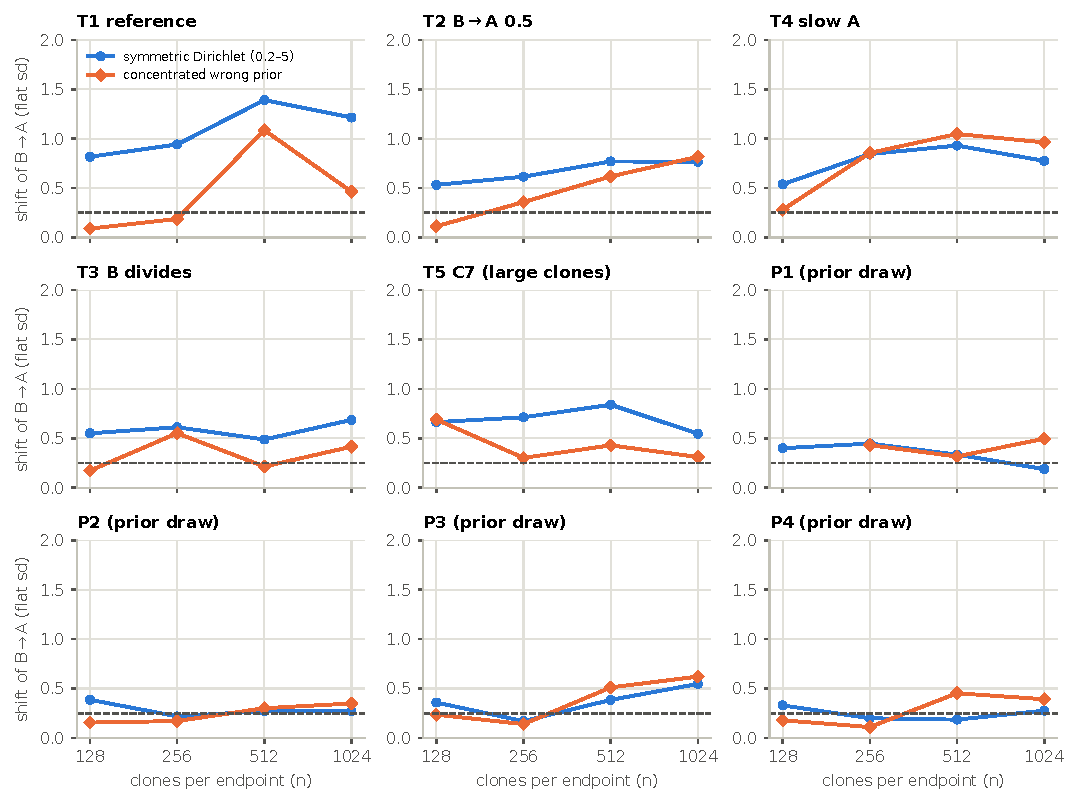
\includegraphics[width=0.62\textwidth]{prior_shift.pdf}

{\small Largest shift of the posterior mean of \BA{} under reliable reweightings, in posterior sd. Dashed: 0.25 sd.}
\end{frame}

\begin{frame}{Backup: the exact Jeffreys prior is not neutral}
\centering
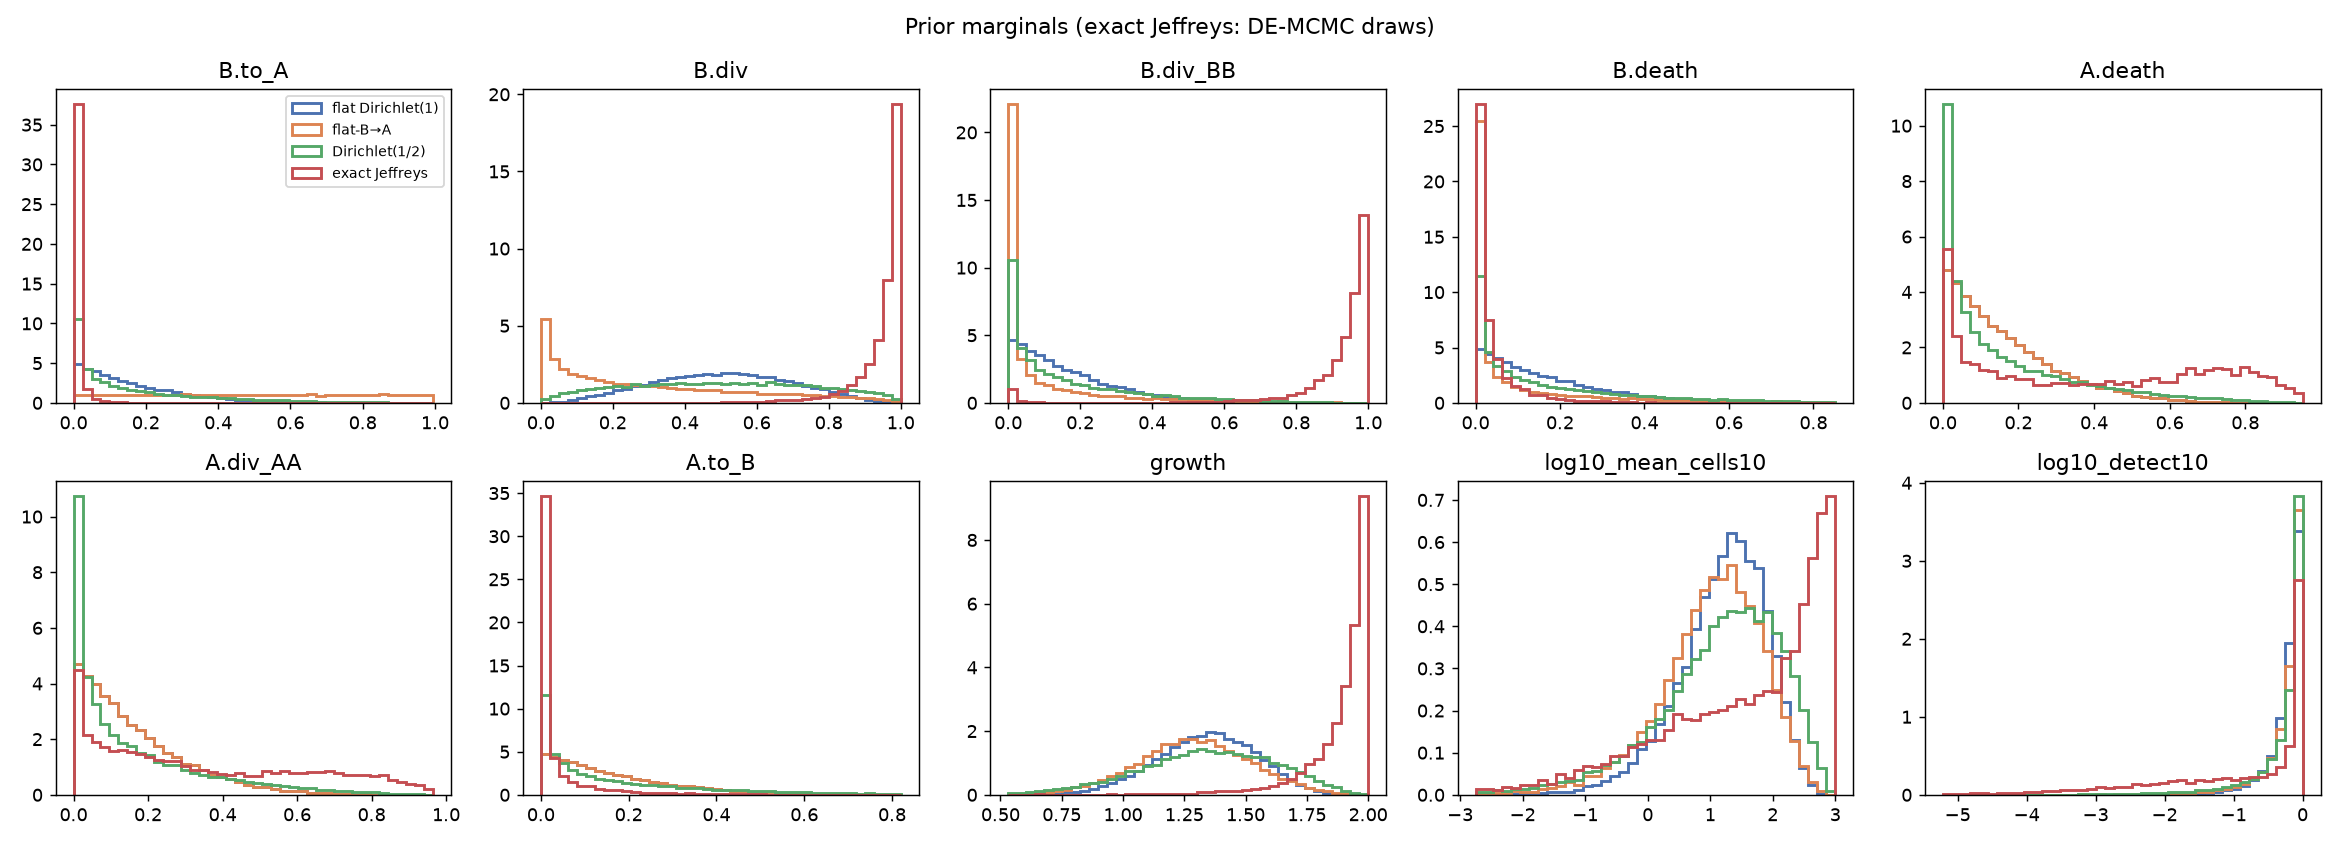
\includegraphics[width=0.97\textwidth]{prior_marginals.png}

{\small Jeffreys puts its mass where clones are most informative: B divides into BB (median 0.97), fast growth, \BA{} $\approx$ 0 (median 0.002).}
\end{frame}

\begin{frame}{Backup: RMSE and coverage by prior}
\centering
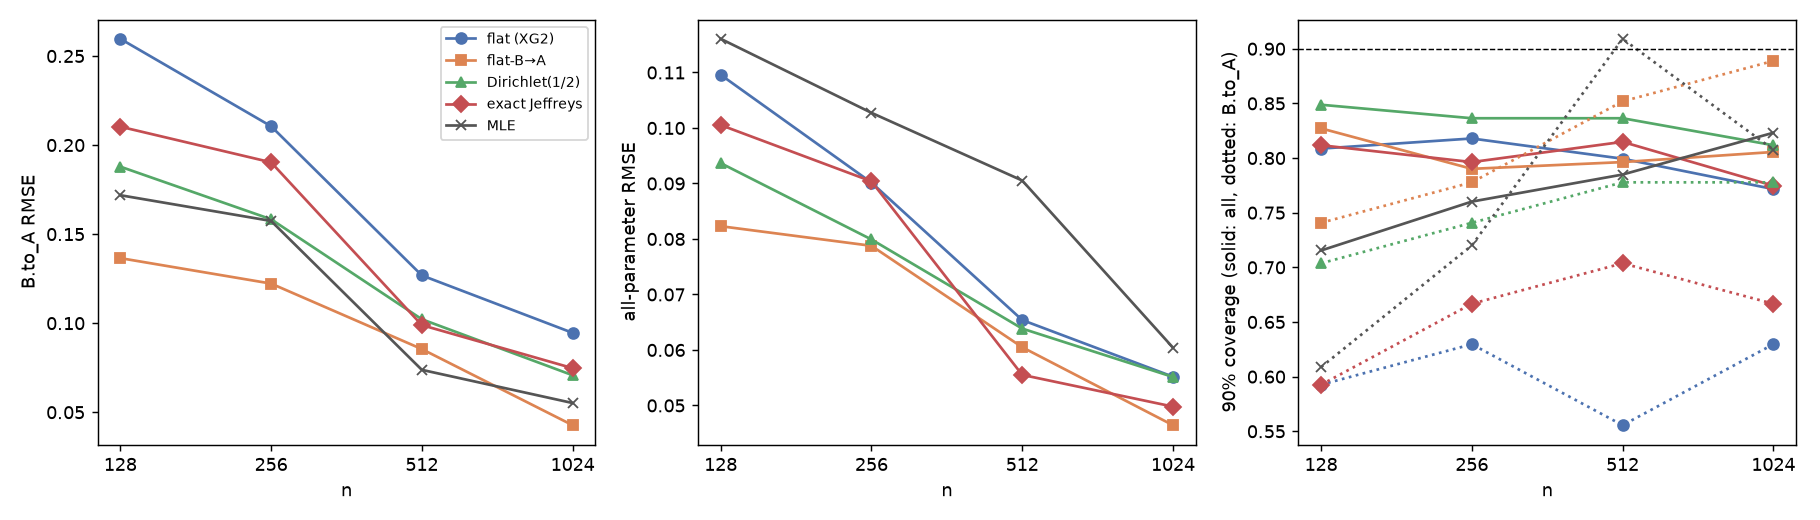
\includegraphics[width=0.97\textwidth]{rmse_coverage_by_n.png}
\end{frame}

\begin{frame}{Backup: large-sample regime}
\centering
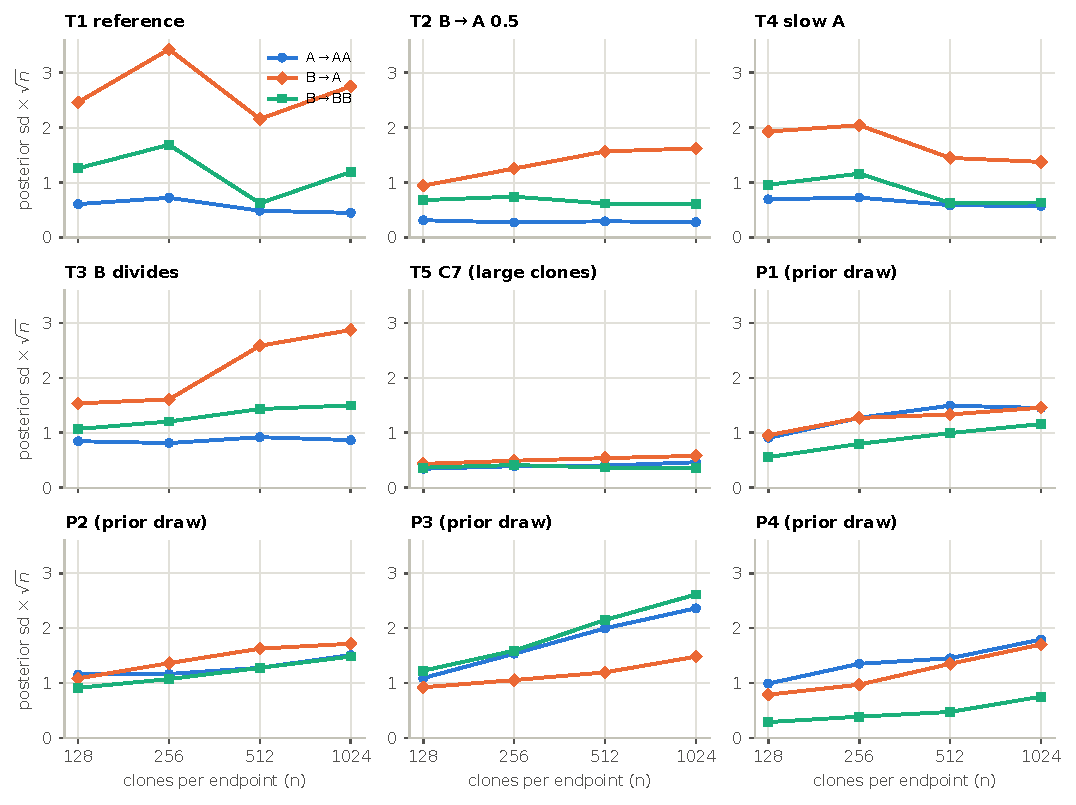
\includegraphics[width=0.62\textwidth]{sd_sqrt_n.pdf}

{\small Posterior sd $\times\sqrt n$: flat = Bernstein--von Mises regime. A's self-renewal by 256--512; \BA{} and B's divisions mostly not by 1024.}
\end{frame}

\begin{frame}{Backup: mis-typing and the dedifferentiation test}
\centering
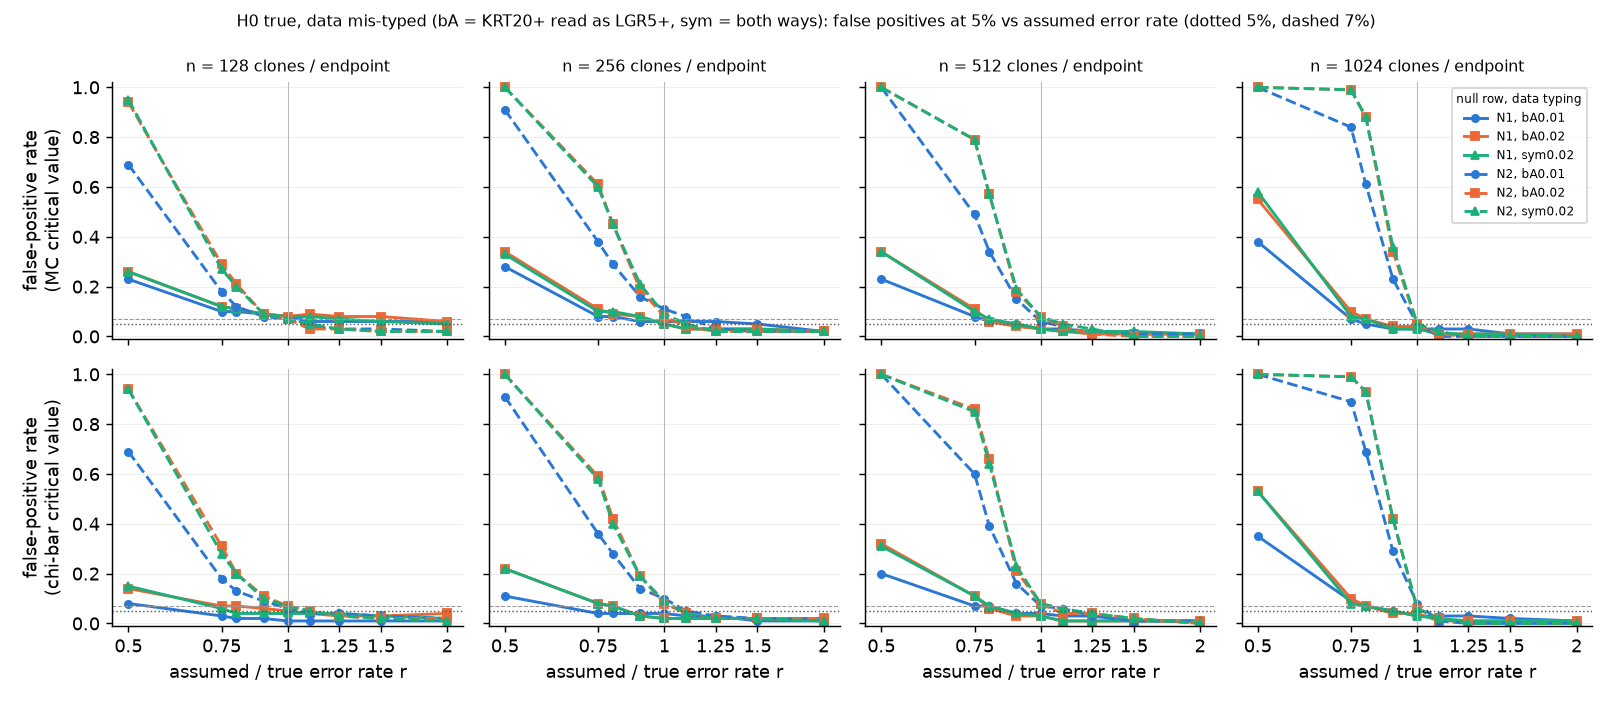
\includegraphics[width=0.95\textwidth]{ratio_fpr.png}

{\small False positives vs assumed / true typing-error rate $r$. Solid: B dies or persists; dashed: B also self-renews.}
\end{frame}

\begin{frame}{Backup: optimal designs per truth}
\centering
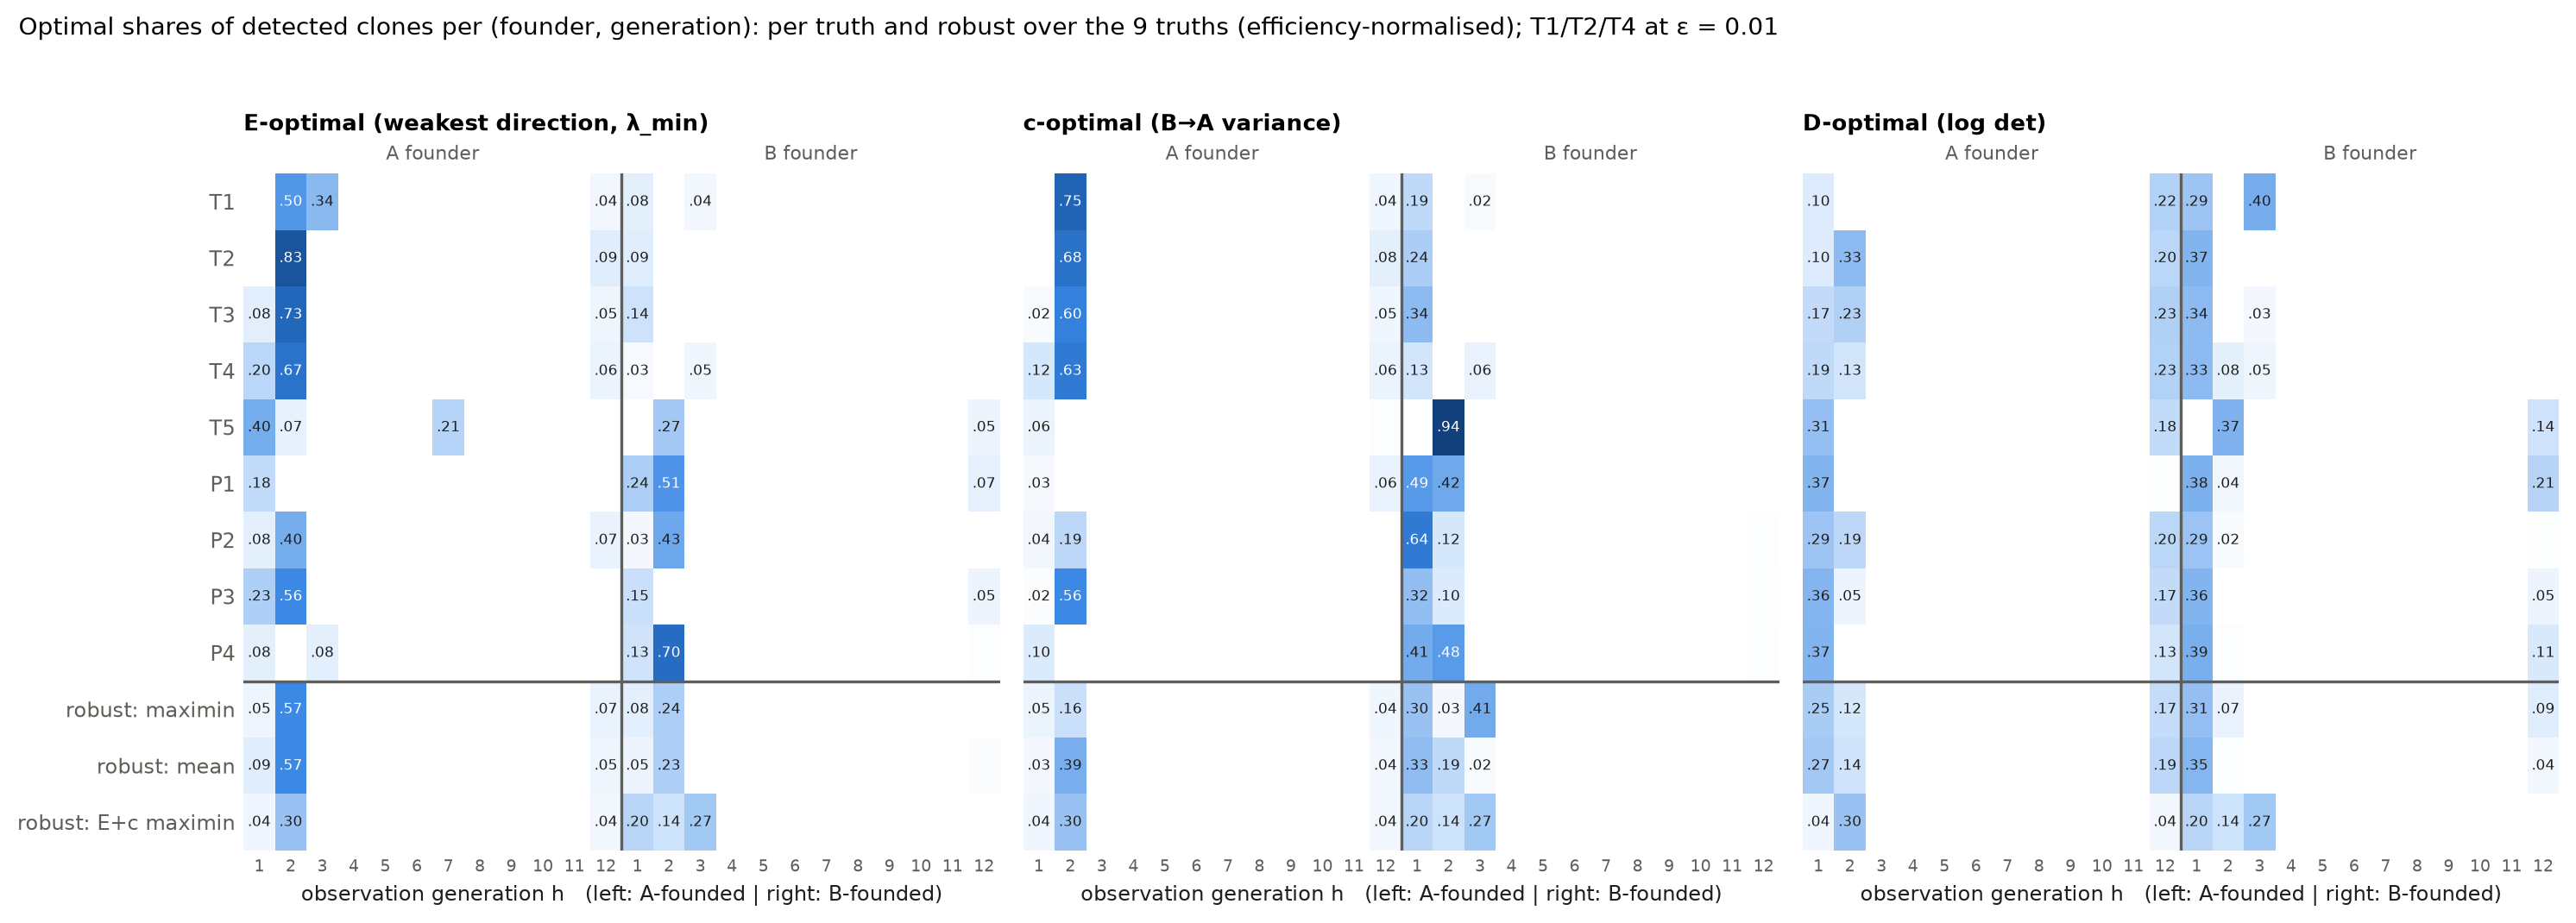
\includegraphics[width=0.97\textwidth]{optimal_weights.png}
\end{frame}

\begin{frame}{Backup: sampler cost}
\small
\begin{itemize}
\item 200--600k gradient evaluations per run (tree depth 5.5--7): NUTS crawls along the weak directions
\item reverse-mode (adjoint) kernel: 4--5$\times$ cheaper per evaluation, identical values; one run 2205\,s $\to$ 414\,s
\item 9/108 runs with $\hat R > 1.05$: 6 were slow (fixed by 8 chains), 3 truly bimodal
\item T1 at $n$ = 1024: a second ``B divides'' branch holds 17\% of the mass (SMC evidence); single NUTS runs put 2--28\% there $\Rightarrow$ report branch masses
\item GPU prototype: only 2.5--3$\times$ over 2 CPU threads (float64), not pursued
\end{itemize}
\end{frame}

\end{document}
